\documentclass[a4paper, 12pt]{article}

\usepackage{graphicx}
\graphicspath{ {../Images/} }
\usepackage[utf8]{inputenc}
\usepackage[T1]{fontenc}
\usepackage{textcomp}
\usepackage{amssymb}
\usepackage{newtxtext} \usepackage{newtxmath}
\usepackage{amsmath, amssymb}
\newtheorem{problem}{Problem}
\newtheorem{example}{Example}
\newtheorem{lemma}{Lemma}
\newtheorem{theorem}{Theorem}
\newtheorem{problem}{Problem}
\newtheorem{example}{Example} \newtheorem{definition}{Definition}
\newtheorem{lemma}{Lemma}
\newtheorem{theorem}{Theorem}


\begin{document}

    

\pagebreak

\section{Clase 1}

\subsection{Info de la materia}

\textit{Mail del profesor.} daniel.penazzi@unc.edu.ar

\textit{Temas a ver.}

\begin{itemize}
    \item Coloreo de grafos 
    \item Flujos en network 
    \item Matchings 
    \item Códigos de correción de errores
    \item P-NP (Complejidad computacional)
    \item Inteligencia artifical
\end{itemize}

La materia tiene tres partes: teórico, práctico y proyecto de programación. Solo
la parte práctica tiene promoción (se explica abajo). El final tiene parte
teórica y parte práctica. La parte teórica es demostrar uno de tres teoremas
dados a priori. La parte práctica tiene ejercicios de demostración o pensamiento
y de resolución de problemas.

La parte práctica se promociona si se aprueban los dos parciales, con cualquer
nota $\geq 4$. De promocionarlo, la parte práctica del final no es necesaria.

El proyecto de programación tiene dos partes. La primera es leer un grafo y
cargar los datos al programa. La segunda es un problema de coloreo de grafos. La
fecha de entrega de la parte uno es en dos o tres semanas a partir de hoy
(13/03). La parte importante es la parte 2.

La biliografía está en el programa 2023.

\subsection{Grafos}

\begin{definition}
    Una grafo es una $2$-upla $G = (V, E)$ con $V$ un conjunto cualquiera (finito) y $E
    \subseteq \left\{ A \subseteq V : |A| = 2 \right\} $
\end{definition}


\small
\begin{quote}

\textbf{Nota.} La restricción de finitud es sólo de esta materia. 

\end{quote}
\normalsize

\begin{center}
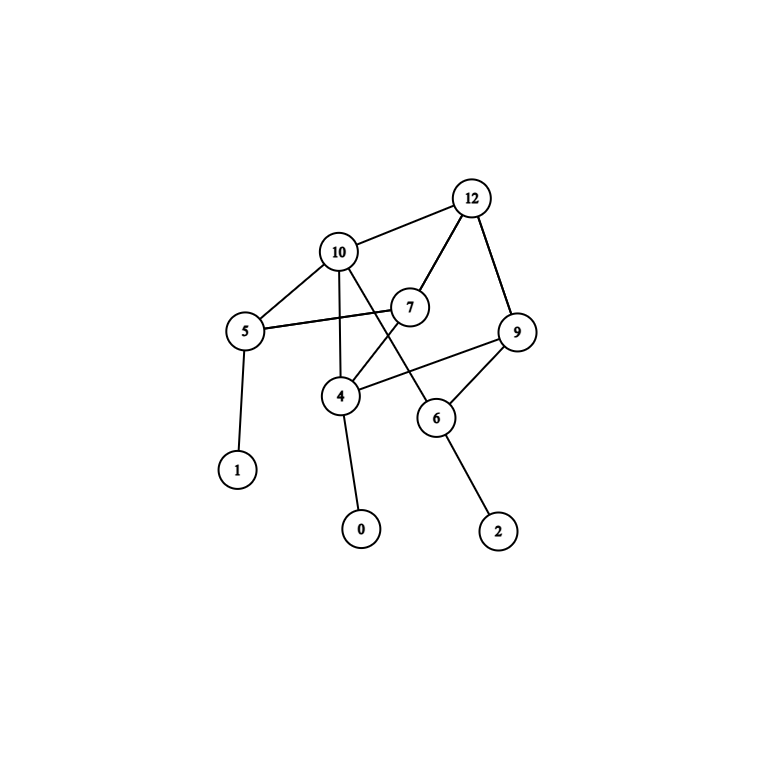
\includegraphics[scale=0.5]{graph}
\end{center}

Los elementos de $V$ se llaman vértices o nodos. Los elementos de $E$ se llaman
lados o aristas. Por convención, a menos que digamos lo contrario, es que $|V| =
n$ y $|E| = m$.

\begin{definition}
    Un camino en un grafo $G = (V, E) $ es una sucesión de vértices $v_1,
    \ldots, v_r$, con $ v_i \in V$ para todo $i$, tal que $\left\{ v_j, v_{j+1}
    \right\} \in E $ para todo $1 \leq j < r$. 
\end{definition}


Dado un camino $v_1, \ldots, v_r$, si $v_1 = x, v_r = y$, decimos que es un
camino de $x$ a $y$. Para todo $G = (V, E)$ definimos la relación binaria 

$$\sim ~:=\left\{ (x, y) \in V^2 : \text{ existe un camino de $x$ a $y$ }  \right\} $$

Es decir, $x \sim y$ denota la relación de que existe un camino entre $x$ e $y$.
Es trivial comproabar que $\sim$ es una relación de equivalencia. Cada clase de
equivalencia $a / \sim$ con $a \in V$ se llama una componente conexa de $G$.

\begin{definition}
    Decimos que $G = (V, E) $ es conexo si y solo si tiene una sola componente
    conexa. Es decir, si $|V / \sim | = 1$.
\end{definition}


\small
\begin{quote}

El profesor no mencionó esto pero es lindo recordar (si alguien ha cursado
lógica) que el conjunto de clases de equivalencia $A / R$ de un conjunto a sobre
una relación binaria $R$ puede en sí mismo darse como un grupo de grafos
disconexos. Por ejemplo, abajo se dan los grafos de un espacio cociente con
siete clases de equivalencia; cada par de vértices unidos por un lado
corresponde a dos elementos equivalentes.


\begin{center}
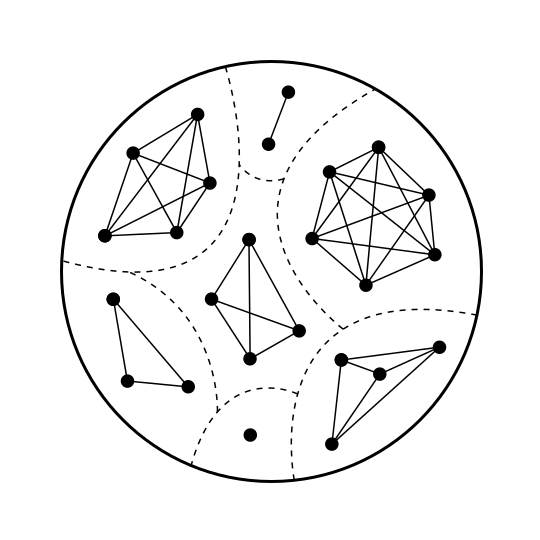
\includegraphics[scale=0.25]{equiv}
\end{center}

Fíjense que de esto se sigue un dato curioso (aunque tal vez irrelevante): Si
$G = (V, E) $ es un grafo conexo con $n$ vértices, el grafo que describe la clase de
equivalencia de $V$ es $K_n$.

\end{quote}
\normalsize

\begin{definition}
    Decimos que un grafo $H = (W, F)$ es un subgrafo de $G =(V, E)$ si
    $W \subseteq V, F \subseteq E$.
\end{definition}

A veces usamos $H \subseteq G$ para decir "$H$ es un subgrafo de $G$", pero no
debe entenderse por esto que $H$ y $G$ son conjuntos.

Observe que no todo $W \subseteq V, F \subseteq E$ satisfacen que $(W, F)$ es un
grafo. Por ejemplo, si $F = \emptyset$ tenemos $F \subseteq E$, pero $F$
no cumple la propiedad de que todos sus elementos sean conjuntos con cardinalidad $2$.

\begin{definition}[Densidad]
    Decimos que un grafo es denso si $m = O(n^2)$. Decimos que un grafo es raro
    si $m = O(n)$.
\end{definition}


\small
\begin{quote}

\textbf{Random fact}. Recuerde que "raro" no sólo significa "inusual" sino que es el
antónimo de "denso". La etimología inglesa es más interesante:
La palabra \textit{Weird} (raro) significaba, en la edad media, destino. Por
eso, en la balada medieval \textit{True Thomas}, se lee "Weird shall never
daunton me": El destino nunca ha de asustarme. Se debe a una antigua leyenda
nórdica en la cual las \textit{Weird sisters}, diosas terribles, tejían el
destino de los hombres. Si le da curiosidad:

https://en.wikipedia.org/wiki/Three_Witches

\end{quote}
\normalsize

\begin{definition}
    Dado $G = (V, E) $, si $x \in V$, $\Gamma(x) := \left\{ y \in V : \left\{ x,
        y\right\}  \in E
\right\} $ se llama el vecindario de $x$. 
\end{definition}

Si $y \in \Gamma(x)$, decimos que $y$
es un vecino de $x$.  El grado de $x$, denotado $d(x)$, es la cantidad de
vecinos de $x$; es decir, $d(x) = |\Gamma(x)|$.
Usamos $\delta = \min \left\{ d(x) : x \in V \right\} $ y $\Delta = \max \left\{
d(x) : x \in V\right\} $. Si $\delta = \Delta$ se dice que $G$ es regular. Por
ejemplo, los
grafos cíclicos y los completos son regulares.

\begin{definition}
    Dado un grafo $G = (V, E) $, decimos que $G$ es regular si $d(x) = d(y)$
    para todo $x, y \in V$.
\end{definition}

Es decir, un grafo es regular si todo vértice tiene la misma cantidad de
vecinos.



\subsection{Repaso de BFS y DFS}

\textit{A completar.}






\subsection{Los grafos $K_n$ y $C_n$}
\label{famosos}

\begin{itemize}
    \item $K_n$ : El grafo completo en $n$ vértices se define 

        $$K_n = \left( \left\{
        1, 2, \ldots, n\right\}, \left\{ \left\{ x, y \right\}  : x, y \in \left\{ 1, 2, \ldots, n
    \right\}  \right\}   \right) $$

    Es el grafo de $n$ elementos donde todos los vértices están conectados unos
    con otros. Resulta que que $m = \binom{n}{2}$. Lo cual implica que $m =
    O(n^2)$.

    \item  $C_n$: El grafo cíclico 

        $$C_n = \left( \left{ 1, 2, \ldots, n \right},
        \left\{ 12, 23, 34, \ldots, (n-1)n, n1 \right\}   \right)$$

        Una observación es
        que $C_3 = K_3$; pero de allí en adelante difieren.
\end{itemize}

\subsection{Coloreo de grafos}

\begin{definition}
    Un coloreo propio de $G = (V, E) $ con $k$ colores es una función  

    \begin{align*}
        C : V \mapsto A
    \end{align*}

    con $|A| = k$ y tal que $xy \in A\Rightarrow C(x) \neq C(y)$.
\end{definition}

Intuitivamente, un coloreo asigna $k$ propiedades a los vértices de modo tal que
ningún par de grafos adyacentes cumple la misma propiedad. 

\small
\begin{quote}

\textbf{Nota.} Hace unos meses escrbí un algoritmo de coloreo en C. Es el
segundo algoritmo dado en esta entrada: 

https://slopezpereyra.github.io/2023-10-29-Hamiltonian/

No prometo que sea muy prolijo o esté bien explicado; ya en general uno es tonto
y encima de tonto no sabe de grafos. Pero tal vez a alguien le sirva, qué se yo.

\end{quote}
\normalsize


\begin{definition}
    El número cromático de un grafo $G= (V, E) $ es 

    \begin{align*}
        \chi(G) = \min_k \left( \exists \text{ coloreo propio de $G$ con $k$
        colores} \right) 
    \end{align*}
\end{definition}

No se conoce un algoritmo polinomial que calcule $\chi(G)$. El proyecto será dar
un algoritmo polinomial que se aproxime a $\chi$.

\subsection{Un algoritmo greedy de coloreo}
~ ~ 

Damos un algoritmo que colorea un grafo $G$ con vértices $v_1, \ldots, v_n$ y
colores $ c_1, c_2, \ldots, c_n  $. Para que el algoritmo
funcione, los colores y los vértices deben tener un orden (en nuestro caso
dado por los subíndices).


\begin{quote}

\textbf{Invariante del algoritmo.} Los coloreos parciales son propios. Es decir,
a medida que se va coloreando iterativamente el grafo, en cada paso el coloreo
resultante debe ser propio.

\textbf{Pasos del algoritmo}. 

\textit{(1)} $C(v_1) = c_1$.

\textit{(2)} $C(v_k) = $ mínimo color que mantenga un coloreo propio (que
satisfaga el invariante).

\end{quote}


\begin{center}
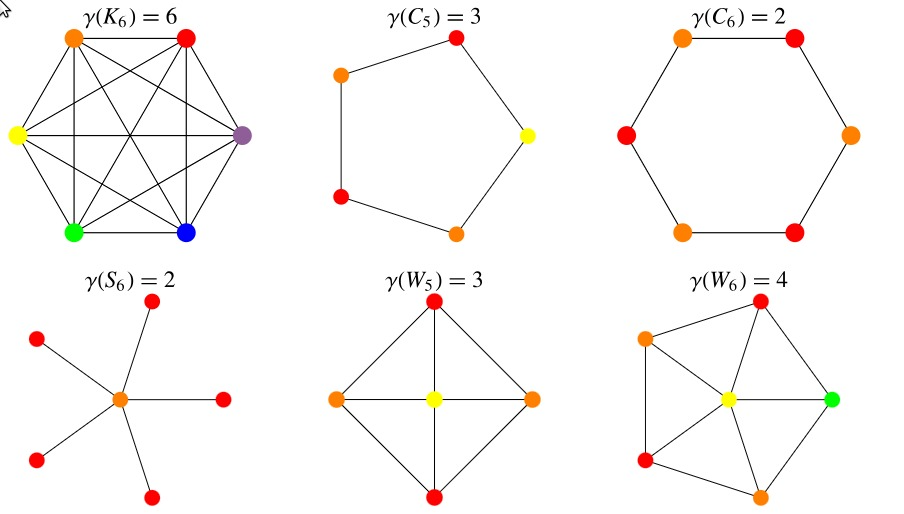
\includegraphics[scale=0.35]{coloring}
\end{center}

\subsection{Acotando $\chi$}

Generalmente nos interesa encontar $\chi(G)$ dado un grafo $G = (V, E) $. Damos
unas pautas y observaciones generales para acotar $\chi(G)$ y así facilitar su
hallazgo.

\begin{lemma}
    Si existe un coloreo propio de $G = (V, E)$ con $k$ colores, entonces
    $\chi(G) \leq k$.
\end{lemma}


\small
\begin{quote}

\textbf{Proof.} Es trivial por definición de $\chi$ ($\chi$ es el mínimo $k$ en
el conjunto de los coloreos posibles de $G$ con $k$ colores).

\end{quote}
\normalsize

El lema significa que para acotar $\chi$ por arriba solo basta dar un coloreo
con $k$ colores.

\begin{lemma}
    Si $H$ es un subgrafo de $G$, $\chi(H) \leq \chi(G)$.
\end{lemma}

Este lema nos dice que podemos acotar $\chi$ por abajo si encontramos un
subgrafo de $G$ cuyo número cromático es conocido. Es fácil ver que $\chi(K_r) =
r$ para todo $r > 1$. Es menos directo pero en clase se demostró que

\begin{align*}
    \chi(C_r) = \begin{cases}
        2 & r \equiv 0 \mod 2  \\ 
        3 & r \equiv 1 \mod 2 
    \end{cases}
\end{align*}

Esto, en combinación con el último lema, nos dice que podemos acotar $\chi(G)$
por abajo simplemente observando si $G$ contiene algún $C_r$  o $K_r$ como
subgrafo. En el caso $C_r$, la cota inferior dada en el caso par, con $\chi(C_r)
= 2$, es trivial (todo grafo necesita al menos dos colores). Por eso nos
quedamos con el siguiente teorema: 

\begin{theorem}
    Sea $G = (V, E) $ un grafo. Si $C_r \subseteq G$ con $r$ impar entonces
    $\chi(G) \geq 3$. Si $K_r \subseteq G$ entonces $\chi(G) \geq r$.
\end{theorem}

\begin{theorem}
    
    Sea $G = (V, E) $ un grafo. Entonces 

    $$\chi(G) = \max \left\{ \chi(C) : C \text{ es componente
conexa de  } G \right\} $$

\end{theorem}


\begin{theorem}
    Sea $G = (V, E) $ un grafo. Entonces $G$ contiene un ciclo impar si y solo
    si $\chi(G) \geq 3$.
\end{theorem}

\small
\begin{quote}

\textbf{Proof.} $(\Rightarrow)$ Trivial. 

$(\Leftarrow)$ Damos una prueba algorítmica. La prueba es simple, pero debe
tenerse presente que usamos \textbf{tres} grafos diferentes en ella: el grafo
$G = (V, E) $ del teorema, una componente conexa $C \subseteq G$, y un grafo
$\mathcal{B} \subseteq C$ resultante de correr BFS de a partir de un vértice de
$C$. El algoritmo determina si $\chi(G) = 2$ y de no serlo construye un ciclo
impar. Usamos la notación $n(z)$ si $z \in V$ para denotar el nivel de $z$ en
$\mathcal{B}$. Dividimos la prueba en tres partes.

\textit{(1)} Como $\chi(G) = \max \left\{ \chi(C) : C \text{ es componente
conexa de  } G \right\} $, tenemos que 

\begin{align*}
    \chi(G) \geq 3 \Rightarrow\exists \text{ c.c. $C$ tal que } \chi(C) \geq 3
\end{align*}

Elegimos $x \in C$ y corremos BFS a partir de él, generando un subgrafo
$\mathcal{B} \subseteq C$ con todos los vértices de $C$ (pero no todos los
lados).

\textit{(2)} Coloreamos cada vértice de $C$ como sigue: como sigue: $c(z)$ será el nivel
BFS de $z$ módulo 2. Esto equivale a hacer $c(x) = 0$ y cada vez que $y$ agrega
a $z$ a la cola de BFS, hacer $c(z) =  1 - c(y)$.

Esto da un coloreo con $2$ colores, pero podría no ser propio (por ejemplo, dos
vecinos de la raíz que son vecinos entre sí tendrían ambos color $1$). Por lo
tanto verificamos si es propio o no. 

\textit{(3)} Si es propio tenemos un coloreo propio de dos colores y $\chi(G) =
2$. Si es impropio, construiremos un ciclo impar. En particular, si no es
propio, existen $u, v \in V$ tales que $c(u) = c(v) $ y $uv \in E$. Pero si
$c(u) = c(v)$, entonces

\begin{align*}
    n(u) \equiv n(v) \mod 2
\end{align*}

Pero en un árbol siempre existe un camino
de la raíz a cualquier vértice arbitrario. Entonces, en $\mathcal{B}$ existe un
camino desde $x$ hasta $u$, y existe un camino desde $x$ hasta $v$. En
particular, existe un vértice $z$ que está en ambos caminos y a partir del cual
los caminos se separan (note que puede ser $x$). Pero en $C$, $uv$ forman un
lado. Luego, en $C$ tenemos el ciclo $z, u, v, z$. 

¿Cuántos lados tiene el ciclo? Vea que de $z$ a $u$ hay $n(u) - n(z)$
lados. De $u$ a $v$ un solo lado, y de $v$ a $z$ otra vez $n(v) - n(z)$.
En total, hay 

\begin{align*}
     n(u) + n(v) - 2 n(z) + 1
\end{align*}

lados. Pero $n(u) \equiv n(v) \mod 2$ y su suma
es par. Luego la suma anterior es impar. Luego existe un ciclo impar en $G$.

\end{quote}
\normalsize

\end{quote}
\normalsize

\begin{theorem}
    Para todo gafo $G = (V, E) $, $\chi(G) \leq \Delta + 1$.
\end{theorem}


\small
\begin{quote}

\textbf{Proof.} $\mathscr{G}$ siempre colorea con $\Delta + 1$  colores o menos. Tome
cualquier orden $v_1 \ldots v_n$ sobre $V$. Para colorear $v_i, i \neq 1$, se
mira el color de los vecinos de $v_i$ que son anteriores en el orden.

El peor caso posible es que todos los vecinos sean anteriores en el orden y
todos tengan colores distintos. En ese caso, $\mathscr{G}$ descarta $d(v_i)$ colores.
Como $d(v_i) \leq \Delta$, entonces $\mathscr{G}$ descarta a lo sumo $\Delta$ colores.
Por lo tanto, siempre habrá al menos un color disponible en $\left\{ 1, 2,
\ldots, \Delta, \Delta + 1 \right\} $.
$\blacksquare$

\end{quote}
\normalsize

Una pregunta natural es si hay grafos cuyo número cromático alcanza la cota
$\Delta + 1$. La respuesta es sí: a saber, 

\begin{itemize}
    \item $\chi(K_n) = n$ y $\Delta = n - 1$.
    \item $\chi(C_{2r+1}) = 3$ y $\Delta = 2$.
\end{itemize}

El siguiente teorema establece que, de todos los grafos conexos, $K_n$ y
$C_{2r+1}$ son los únicos que alcanzan la cota.

\begin{theorem}[Brooks]
    Sea $G = (V, E) $ un grafo conexo distinto de un $K_n$ y un $C_{2r + 1}$.
    Entonces $\chi(G) \leq \Delta$.
\end{theorem}


\small
\begin{quote}

\textbf{Proof.} Complicada, una hora y media o dos de hacer. Triste.

\end{quote}
\normalsize

\begin{theorem}[Baby Brooks o Brooks para bebés]
    Si $G = (V, E) $ un grafo conexo y no regular, entonces $\chi(G) \leq
    \Delta$.
\end{theorem}


\small
\begin{quote}

\textbf{Proof.} Es un caso particular del teorema de Brooks. Corramos BFS$(x)$
con $d(x) = \delta$.
Como $G$ es conexo, obtenemos todos los vértices. Pues los vértices son
agregados iterativamente al árbol del BFS, existe un orden dado precisamente por
el orden de inserción al árbol.

Daremos un orden (que no es el anterior) tal que $\mathscr{G}$ colorea $G$ con a lo
sumo $\Delta$ colores. En particular, es el orden inverso al anterior. Es decir
que el último elemento del orden es la raíz $x$.

Como siempre el color del primer elemento es $1$. Sea $z \neq v_1$ (en el orden
del $\mathscr{G}$). El peor caso posible, que $z$ tenga como vecinos a todos los
anteriores, es imposible aquí, porque en el orden de DFS todo $y \neq x$ es
insertado en el árbol por un vértice que ya estaba en el árbol. Y ese vértice
debe ser un vecino. Es decir, en el orden de inserción del BFS, todo vértice
tiene un vecino que es anterior en el orden. Entonces, en el orden inverso, todo
$y \neq x$ tiene al menos un vecino posterior. Entonces, en el peor de los
casos, tiene $d(y) - 1$ vecinos anteriores. Por lo tanto, greedy elimina a lo
sumo $d(y) -
1 \leq \Delta - 1$ colores. $\therefore $ Siempre puede colorear a $y$ con un
color en $\left\{ 1, 2, \ldots, \Delta \right\} $.

Cuando llega a $x$, $\mathscr{G}$ elimina a lo sumo $d(x) = \delta$ colores. Y como $G$
no es regular, $\delta < \Delta$. $\therefore $ Existe al menos un color para
$x$ en $\left\{ 1, 2, \ldots, \Delta \right\} $.

\end{quote}
\normalsize


\subsection{¿Para qué acotar $\chi$? Para encontar $\chi$!}

En general no es fácil mostrar que $\chi(G) = \varphi$ de manera directa. Uno
puede mostrar entonces que $\varphi_{l} \leq \chi(G) \leq \varphi_{u}$ usando
las acotaciones vistas antes. Si sucede que $\varphi_l = \varphi_u$ qué bonito
hemos encontrado $\chi(G)$. Si este no es el caso de igual modo estamos
restringiendo el espacio de soluciones posibles. Por ejemplo, si $3 \leq \chi(G)
\leq 4$, tenemos que $\chi(G) = 3$ o $\chi(G) = 4$, y a veces es fácil ver (y
demostrar) cuál de los casos es correcto.

\pagebreak

\subsection{Limitaciones de $\mathscr{G}$}


\textbf{Ejemplo de $\mathscr{G}$ mal.} Sea $G = (V, E)$ un grafo tal que $n = 2i$ es par
y 

\begin{align*}
    E = \left\{ xy : x \text{ impar }, y \text{ par }, y \neq x + 1\right\} 
\end{align*}

El grafo es claramente bipartito (un par nunca se conecta con un par, un impar
nunca con un impar) y tiene un coloreo de 2 colores. Sin embargo, al correr
$\mathscr{G}$ sobre este grafo, obtenemos un coloreo sub-óptimo.

Se deja al lector verificar los coloreos sub-óptimos que resultan si $n = 2, 4,
6$. Se presenta la siguiente hipótesis inductiva haciendo inducción sobre $i$:


\small
\begin{quote}

\textit{Hipótesis inductiva}. Para todo $j \leq k$, $\mathscr{G}$ colorea el grafo con
$c(2j - 1) = c(2j) = j$ colores.

\end{quote}
\normalsize

\small
\begin{quote}

    \textit{Caso inductivo.} Si $j \leq k$ por $HI$ tenemos $c(2j - 1) = c(2j) =
    j$. Si $j = k + 1$, tenemos que $2(k+1) - 1$ es impar y forma lados con
    todos los pares anteriores. Luego greedy no puede asignarle el color de
    ningún par anterior. Es decir, no puede asignar ningún color entre $1$ y
    $k$. Luego greedy lo colorea con $k + 1$. El mismo razonamiento muestra que
    el vértice $2(k+1)$ se colorea con $i + 1$.

    Por lo tanto, greedy colorea $G$ con $\frac{n}{2}$ colores.


\end{quote}
\normalsize


\subsection{Hill clmbing}

Hill climbing es un algoritmo de optimización matemática. Dada una función $f :
\mathbb{R}^n \to \mathbb{R}$ que se quiere maximizar, el algoritmo toma un punto
arbitrario
$\vec{x} \in \mathcal{D}_f$ y evalúa $f(\vec{x})$. Luego se hace $\Delta\vec{x} =
(x_1, \ldots, x_{i} + \epsilon, \ldots, x_n)$ con $\epsilon \in R$ e $i$
arbitario y se vuelve a testear. Si la función incrementa, se hace
$\vec{x} = \Delta\vec{x}$: si no, se hace la modificación inversa. Este proceso
se repite iterativamente hasta que un criterio es satisfecho.

El principal problema del algoritmo de Hill climbing es que encuentra solo
óptimos locales. Para lidiar con este problema, se usa \textit{simulated
annealing}. Si $\Delta \vec{x}$ va mejor se lo acepta; pero si $\Delta \vec{x}$
va peor se otorga una cierta probabilidad de aceptarlo de todos modos. La
probabilidad de aceptar va reduciendo con el tiempo. La idea es permitir la
salida de optimos locales con el tiempo.

En coloreo de grafos, Hill climbing toma la siguiente forma. Se prueba un orden
de $V$ arbitrario y se lo colorea con $\mathscr{G}$. Luego hacer una pequeña
permutación y se prueba de nuevo, etc. 

Existe un modo de asegurarnos que la mutación $\Delta \vec{x}$ de $\vec{x}$
nunca empeore (puede permanecer igual). El problema es que para hacer esto,
reducimos el espacio de búsqueda; es decir, las permutaciones que
exploraremos (las que no pueden empeorar el rendimiento) son muy pocas, y puede
ser que ninguna mejore el rendimiento. 

Una forma de lidiar con esto es elegir varios órdenes iniciales al azar y
aplicar esta idea a cada una de ellas.

\begin{theorem}[VIT]

    Sea $G = (V, E) $ un grafo con un coloreo propio $c$ con $r$ colores $c_1,
    \ldots, c_r$. Sea $V_{c_i} := \left\{ x \in V : c(x) = c_i \right\} $. Sea $P$
    una permutación de $c_1, \ldots, c_r$. Es claro que $P : \left\{ c_1, \ldots, c_r
    \right\} \mapsto \left\{ c_1, \ldots, c_r \right\} $ es una biyección.


    Ordenemos los vértices poniendo primero los vértices de $V_{P(c_1)}$; luego
    los de $V_{P(c_2)}$, etc. Es decir, ordenamos los vértices por bloques de
    color. Entonces $\mathscr{G}$ con ese orden usa a lo sumo $r$ colores.
    
\end{theorem}


\small
\begin{quote}

\textbf{Proof.} Hacemos inducción sobre $r$. 

\textit{Caso base $i = 1$.} Los vértices de $V_{P(c_i)}$ tienen el mismo color $P(c_i)$.
Porque $c$ es un coloreo propio, y los vértices en cada $V_{P(c_i)}$ no pueden
formar lados entre sí, $\mathscr{G}$ los colorea a todos con el color 1 y usa un color.
$\blacksquare$


$HI(i) \Rightarrow HI(i+1)$: Sea $x \in V_{P(c_1)} \cup  \ldots \cup
V_{P(c_{i+1})}$. Si $x$ está en alguno de los primeros $i$ bloques, $\mathscr{G}$ lo
colorea con uno de entre $i$ colores por hipótesis inductiva. 

Si $x \in V_{P(c_{i+1})}$, el
caso en que $\mathscr{G}$ lo colorea con un color menor o igual a $i + 1$ no viola lo
que queremos demostrar. Pero asumamos que lo colorea con el color $i +
2$. Entonces ningún color menor estaba disponible; entonces $x$ es vecino de
algún $z$ de color $i + 1$. Pero todos los vértices de $V_{P(c_{i})}$ están
coloreados el color $c_i$. Luego $z \in V_{P(c_{i+1})}$. Pero si
tanto $x, z \in V_{P(c_{i+1})}$ entonces $c(x) = c(z) = P(c_{i+1})$, lo cual
implica que $c$ no es propio. $(\bot)$

\end{quote}
\normalsize

\pagebreak 

\section{Redes y flujos}

Una red es un grafo dirigido con un límite en la información o carga
transferible de un nodo a otro. 

El modelo de problema central es una red de productores y
consumidores. Se trata de encontrar el máximo de información (o producto)
transferible de los productores a los consumidores. Lo transferido de
productores a consumidores se llama flujo. Llamamos a este problema \textit{max
flow}.

\begin{definition}
    Un grafo $G = (V, E) $ con $V$ un conjunto y $E \subseteq V \times V$ se
    llama dirigido.
\end{definition}

Usaremos $\overrightarrow{xy}$ para denotar $(x, y)$ donde $(x, y) \in E$. Observe que
$\overrightarrow{xy} \neq \overrightarrow{yx}$.

\begin{definition}
    Una red o network es una $3$-upla $(V, E, c)$ donde $(V, E)$ es un grafo
    dirigido y $c : E \to \mathbb{R}^{+}$ es una función.
\end{definition}

La función $c$ denota la capacidad de cada uno de los lados.

\begin{definition}[Vecinos]
    Definimos $\Gamma^{+}(x) = \left\{ x \in V : \overrightarrow{xy} \in E \right\} $ y,
    por otro lado,
    $\Gamma^{-}(x) = \left\{ y \in V : \overrightarrow{yx} \in E \right\} $
\end{definition}

Usualmente nos preguntamos no cuánta información puede enviarse de un nodo a
otro, sino cuánta puede enviarse de un conjunto de nodos a otro (de una parte
del grafo a otra). Esto inspira la siguiente notación.

\begin{definition}
    Sea $g : E \to \mathbb{R}$ y sean $A, B \subseteq V$. Definimos  

    \begin{align*}
        g(A, B) = \sum_{x \in A, y \in B \text{ t.q. } \exists \overrightarrow{xy} \in E}
        g(\overrightarrow{xy})
    \end{align*}
\end{definition}

Usualmente usamos la siguiente notación: Si $\zeta$ es una expresión booleana,
$[\zeta]$ es su evaluación en $\left\{ 0, 1 \right\} $. Esto a veces facilita
las cosas; por ejemplo, la definición anterior es equivalente a

\begin{align*}
    g(A, B) = \sum_{\overrightarrow{xy} \in E}[x \in A] [y \in B] [\overrightarrow{xy} \in E] g(\overrightarrow{xy})
\end{align*}

\begin{definition}
    Sea $\mathcal{N} = (V, E, c)$ una network. Sea $x \in V$ y $g : E \to
    \mathbb{R}$. Definimos 

    \begin{align*}
        \text{out}_{g}(x) := \sum_{E} [y \in V][\overrightarrow{xy} \in E]g(x) &= g \left(
        \left\{ x \right\}, V  \right) 
    \end{align*}

    Análogamente, 

    \begin{align*}
        \text{in}_g(x) := \sum[y \in V] [\overrightarrow{yx} \in E]g(\overrightarrow{yx}) = g\left( V,
        \left\{ x \right\} \right) 
    \end{align*}
\end{definition}

\begin{definition}
    Dada $\mathcal{N} = (V, E, c)$ una network y $s, t \in V$, una función $f
    :E \to \mathbb{R}$ es un flujo si y solo si 

    \begin{quote}
        
    \begin{enumerate}
        \item $0 \leq f(\overrightarrow{xy}) \leq c(\overrightarrow{xy}) ~ \forall \overrightarrow{xy} \in E$
            (feasability)
        \item $\text{in}_f(x) = \text{out}_f(x) ~ \forall x \in V - \left\{ s, t
            \right\} $ (conservación) 
        \item $\text{out}_f(s) \geq \text{in}_f(s)$ ($s$ es una source o
            productor)
        \item $\text{in}_f(t) \geq \text{out}_f(t)$ (t es un consumidor o sink)
    \end{enumerate}
    \end{quote}

\end{definition}

A veces se pide que lo que entra a $s$ sea cero y lo que salga de $t$ sea cero,
pero esto no es necesario. A fines prácticos, en los ejemplos que veremos esta
última restricción se cumple. Más aún, suele suceder que $\Gamma^{+}(t) =
\emptyset$ y $\Gamma^{-}(s) =\emptyset$.

\begin{definition}
    Sea $\mathcal{N} = (V, E, c)$ una network y $f$ un flujo en $\mathcal{N}$
    de $s$ a $t$. Definimos el valor de un flujo como sigue:

    \begin{align*}
        v(f) = \text{out}_f(s) - \text{in}_f(s)
    \end{align*}
\end{definition}

El valor de un flujo es, por lo tanto. lo que "sale" de $s$ en ese flujo; o
bien, la cantidad total de información que está siendo transferida desde $s$
hacia $t$. Es intuitivo pensar que esto será lo mismo que la cantidad de
información que llega a $t$. El siguiente teorema establece esta equivalencia.

\begin{theorem}
    Sea $\mathcal{N} = (V, E, c)$ una network y $f$ un flujo en $\mathcal{N}$.
    Luego $v(f) = in_f(t) - out_f(t)$.
\end{theorem}


\small
\begin{quote}

    \textbf{Proof.} Observe que 

    \begin{align*}
        f(V, V) &= \sum_{\overrightarrow{xy} \in E} f(\overrightarrow{xy}) \\ 
                &= \sum_{x \in V} \sum_{y \in V, \overrightarrow{xy} \in E} f(\overrightarrow{xy}) \\ 
                &= \sum_{x \in V} out_f(x)
    \end{align*}

    Ahora bien, el mismo razonamiento indica que $f(V, V) = \sum_{x \in V}
    \text{in}_f(x)$. Es decir, 

    \begin{align*}
        \sum_{x \in V} \text{out}_f(x) = \sum_{x \in V} \text{in}_f(x)
    \end{align*}

    Por la propiedad \textit{(2)} de un flujo, tenemos que $in_f(x) = out_f(x)$.
    Cancelando términos en las sumatorias, llegamos a 

    \begin{align*}
        \sum_{x \in V} \text{out}_f(x) &= \sum_{x \in V} \text{in}_f(x) \\ 
        \Rightarrow ~& \text{out}_f(s) - \text{in}_f(s) = \text{in}_f(t) -
        \text{out}_f(t) = v(t) ~ \blacksquare
    \end{align*}
    
    \begin{quote}
        (Incidentalmente, como $\text{out}_f(s) \geq \text{in}_f(s)$, tenemos que
        $v(t) \geq 0$, y por lo tanto $\text{in}_f(t) \geq \text{out}_f(t)$, lo
        cual es la propiedad \textit{(4)} de un flujo.)
    \end{quote}

\end{quote}
\normalsize

\begin{definition}
    Sea $\mathcal{N} = (V, E, c)$ una network y $f$ un flujo en $\mathcal{N}$ de
    $s$ a $t$.
    $f$ se dice maximal si y solo si $v(f) \geq v(g)$ para toda $g$ que sea un
    flujo en $\mathcal{N}$ de $s$ a $t$.
\end{definition}


\begin{lemma}[Un lema obvio]
    Sean $f, g$ funciones sobre los lados con $f(\overrightarrow{xy}) \leq g(\overrightarrow{xy})$
    para toda $\overrightarrow{xy} \in E$. Entonces $f(A, B) \leq g(A, B)$ para todo $A, B
    \subseteq V$.
\end{lemma}

Observemos que si $v(f) = c(\left\{ s \right\}, V)$, entonces $f$ es maximal. Es
el caso en que saturamos completamente la capacidad de $s$. Sin embargo, la
inversa no se cumple: si un flujo es maximal, no necesariamente saturamos los
lados de $s$.

\begin{theorem}[Probar que flujo es maximal]
    Sea $f$ un flujo sobre $\mathcal{N} = (G, E, c)$ de $s$ a $t$. Entonces
    $v(f) = c(\left\{ s \right\}, V) \Rightarrow f$ es maximal.
\end{theorem}


\small
\begin{quote}

\textbf{Proof.} Sea $g$ un flujo en $\mathcal{N} = (V, E, c)$ de $s$ a $t$. Por
popiedad \textit{(1)} de la definición de flujo, $g(\overrightarrow{xy}) \leq c(\overrightarrow{xy})$
para todo $\overrightarrow{xy} \in E$. Por el lema anterior, 

\begin{align*} g(\left\{ s \right\}, V) \leq c( \left\{ s \right\}, V  )\end{align*}

Vea que $v(g) = out_g(s) - in_g(s) \leq out_g(s)$. Pues $out_g(s) = g(\left\{ s
\right\}, v ) \leq c(\left\{ s \right\}, v ) = v(f)$. Obtenemos entonces $v(g)
\leq v(f)$.

\end{quote}
\normalsize

\subsection{Algoritmo $\mathscr{G}$ para flujo}

Damos un algoritmo para encontrar un flujo $f$ sobre una network $\mathcal{N} =
(V, E, c)$. Recordemos que el flujo $f$ de una network es simplemente una
función que asigna valores a sus lados. El algorimo hace lo siguiente:

\begin{quote}

    \textit{(1)} Inicializa el flujo en $f(\overrightarrow{xy}) = 0$ para todo $\overrightarrow{xy}
    \in E$. 

    \textit{(2)} Encuentra un camino no saturado de $s$ a $t$; es decir, un
    camino tal que el flujo es inferior a la capacidad en cada lado. Si el
    camino no existe, termina.

    \textit{(3)} Suma al flujo de cada lado en el camino el valor máximo que
    puede sumarse sin sobrepasar la capacidad de ningún lado.

    \textit{(4)} Regresa a \textit{(2)}.
    
\end{quote}

En pseudo-código, el algoritmo es:


\begin{align*}
    &f(\overrightarrow{xy}) = 0 \text{ for all $\overrightarrow{xy} \in E$ } \\ 
    &\textbf{while} ~ (\exists \text{ camino no saturado de $s$ a $t$ })
    ~\textbf{do}\\
    & ~ ~ ~ ~ \text{Encuentra camino no saturado $sx_0 \ldots x_{r} t$}\\
    &~ ~ ~ ~ \epsilon = \min_{0 \leq i < r} \Big\{ c(\overrightarrow{x_i x_{i+1}}) -
    f(\overrightarrow{x_i x_{i+1}})\Big\}\\
    &~ ~ ~ ~ \textbf{for} ~ i := 0 ~ \textbf{do}\\ 
    &~ ~ ~ ~  ~ ~ ~ ~  f(\overrightarrow{x_i x_{i+1}}) := f(\overrightarrow{x_i x_{i+1}}) + \epsilon \\
    &~ ~ ~ ~ \textbf{od} \\ 
    &\textbf{od}
\end{align*}

Algunas propiedades buenas del algoritmo $\mathscr{G}$ para flujos son las siguientes:

\begin{itemize}
    \item Siempre devuelve un flujo 
    \item Siempre termina, porque en cada iteración satura al menos un lado y
        nunca "desatura" los lados.
    \item Su complejidad $O(m^2)$, porque hace $O(m)$ iteraciones y en cada
        iteración es $O(m)$.
\end{itemize}

Su gran propiedad mala es que no siempre devuelve un flujo maximal. Pero esto
puede resolverse si adaptamos un poco el algoritmo de $\mathscr{G}$. Para dar con la
adaptación adecuada, antes damos una nueva definición. 

\subsection{Algoritmo Ford-Fulkerson}

\begin{definition}
    Un $f$-camino aumentante es una sucesión $x_0, \ldots, x_r$ de vértices tal que
    $x_0 = s, x_r = t$, y para cada $0 \leq i < r$, uno de los dos casos se
    cumplen: 

    \begin{quote}
        
        \begin{itemize}
        \item $\overrightarrow{x_i x_{i+1}} \in E$ y
        $f(\overrightarrow{x_ix_{i+1}}) < c(\overrightarrow{x_ix_{i+1}})$.
    \item $\overleftarrow{x_{i}x_{i+1}} \in E$ y
            $f(\overleftarrow{x_{i}x_{i+1}}) > 0$.
        \end{itemize}
    \end{quote}


\end{definition}
    
La primera condición establece que si un trecho del camino es \textit{forward}
($\overrightarrow{x_i x_{i+1}} \in E$), el flujo circulante en ese trecho es inferior
a su capacidad. La segunda condición establece que si un trecho del camino es
\textit{backward} ($\overleftarrow{x_{i}x_{i+1}} \in E$), el flujo circulante en
ese trecho es mayor a cero. 

\begin{theorem}
    Si $f$ es un flujo de valor $v$, y aumentamos $f$ con un $f$-camino
    aumentante con $\epsilon$, entonces lo que queda sigue siendo un flujo y su
    valor es $v + \epsilon$.
\end{theorem}

La propiedad linda de Ford-Fulkerson es que, si termina, devuelve un flujo
maximal. La propiedad fea es que no siempre termina.

\begin{quote}
\begin{align*}
    &f(\overrightarrow{xy}) := 0 \text{ for all $\overrightarrow{xy} \in E$ } \\ 
    &\textbf{while} ~ (\exists \text{ $f$-camino aumentante $s$ a $t$ })
    ~\textbf{do}\\
    & ~ ~ ~ ~\text{Hallar $f$-camino aumentante $x_0 \ldots x_{r-1}x_r$
    con $x_0 = s, x_{r} = t$}\\
    &~ ~ ~ ~ \textbf{for} ~ i := 0 \textbf{ to } r  \textbf{ do}\\ 
    &~ ~ ~ ~ ~ ~ ~ ~ ~ \epsilon_i := \begin{cases}
        c(\overrightarrow{x_ix_{i+1}}) - f(\overrightarrow{x_ix_{i+1}}) &
        \overrightarrow{x_ix_{i+1}}\in E\\ 
        f(\overleftarrow{x{i}x_{i+1}}) & \overleftarrow{x_{i}x_{i+1}} \in E
    \end{cases} &  \\
    &~ ~ ~ ~ \textbf{od}\\
    &~ ~ ~ ~  \epsilon = \min \left\{ \epsilon_0, \ldots, \epsilon_{r} \right\} \\
    &~ ~ ~ ~ \textbf{for} ~ i := 0 \textbf{ to } r  \textbf{ do}\\ 
    &~ ~ ~ ~ ~ ~ ~ ~ ~ \textbf{if } ~ \overrightarrow{x_ix_{i+1}} \in E \textbf{
    then}\\ 
    & ~ ~ ~ ~ ~ ~ ~ ~ ~ ~ ~ ~ ~ ~ ~ ~ f(\overrightarrow{x_{i}x_{i+1}}) :=
    f(\overrightarrow{x_{i}x_{i+1}}) + \epsilon\\
    & ~ ~ ~ ~ ~ ~ ~ ~ ~  \textbf{else} \\ 
    & ~ ~ ~ ~ ~ ~ ~ ~ ~ ~ ~ ~ ~ ~ ~ ~ f(\overleftarrow{x_{i}x_{i+1}}) :=
    f(\overleftarrow{x_{i}x_{i+1}}) - \epsilon\\
    & ~ ~ ~ ~ ~ ~ ~ ~  \textbf{fi}\\
    & ~ ~ ~ ~ \textbf{od}\\
    &\textbf{od}
\end{align*}

\end{quote}
\normalsize

Como puede observarse, el algoritmo encuentra un camino aumentante arbitrario,
encuentra la menor cantidad de flujo que puede o bien agregarse o bien removerse
de la circulación en cada trecho del camino, y luego lo agrega o lo sustrae en
cada trecho dependiendo del caso.

\subsection{Análisis de Ford-Fulkerson}

\begin{definition}
    Sea $\mathcal{N} = (V, E, c)$ una network. Un corte es un conjunto $S
    \subseteq V$ tal que $s \in S, t \not\in S$.
\end{definition}

\begin{lemma}
    Sea $f$ un flujo sobre una network $\mathcal{N}$ con un corte $S$. Entonces
    $v(f) = f(S, \overline{S}) - f(\overline{S}, S)$.
\end{lemma}


\small
\begin{quote}

\textbf{Prueba.} Recordemos que $out_f (x) - in_f(x) = 0$ si $x \neq s, t$.
Recordemos además que $out_f(s) - in_f(s) = v(f)$ por definición. Entonces 

\begin{align*}
    \sum_{x \in S} \left( out_f(x) - in_f(x) \right) &= out_f(s) - in_f(s) +
    \sum_{x \in S, x \neq s} out_f(x) - in_f(x)  \\ 
                                                     &= out_f(s) - in_f(s) \\ 
                                                     &= v(f)
\end{align*}

Ahora bien, la sumatoria dada puede expresarse de otra forma. Observe que 

\begin{align*}
    \sum_{x \in S} \left( out_f(x) - in_f(x) \right)  &= \sum_{x \in S} \Big[f\left(
    \left\{ x \right\}, V \right) - f(V, \left( x \right) )\Big] \\ 
\end{align*}

Por la definición de $g(A, B)$, si partimos los dos términos dentro de la
sumatoria en dos sumatorias separadas, obtenemos que lo anterior es

\begin{align*}
    f(S, V) - f(V, S) &= f(S, S \cup \overline{S}) - f(S \cup \overline{S}, S)
    \\ 
                      &=\left[ f(S, S) + f(S, \overline{S}) \right]  - \left[
                      f(S, S) + f(\overline{S}, S) \right] 
\end{align*}

En resumen, 

\begin{align*}
    \sum_{x \in S}\left( out_f(x) - in_f(x) \right)  &= f(S, S) + f(S,
    \overline{S}) - f(S, S) - f(\overline{S}, S) \\ 
                                                     &= f(S, \overline{S}) -
                                                     f(\overline{S}, S)
\end{align*}

Combinando ambos resultados, $v(f) = f(S, \overline{S}) - f(\overline{S}, S)$.

\end{quote}
\normalsize

\begin{definition}
    La capacidad de un corte $S$ se define como $Cap(S) = c(S, \overline{S})$.
\end{definition}

Es decir, es la suma de las capacidades de todos los vértices que van desde el
corte hacia fuera del corte.

\begin{definition}
    Un corte $S$ es minimal si su capacidad es menor o igual a la de todo otro
    corte.
\end{definition}

\begin{theorem}[Max flow, min cut]
    Sea $S$ un corte arbitrario sobre una network $\mathcal{N} = (V, E, c)$ con
    flujo $f$. Luego $v(f) \leq Cap(S)$. Más aún, $f$ es maximal si y solo si
    existe un corte minimal $\mathcal{S}$ tal que $v(f) =
    Cap(\mathcal{S})$.
\end{theorem}


\small
\begin{quote}

\textbf{Prueba.} \textit{(1)} Probaremos que $f \leq Cap(S)$ para un corte $S$ y
un flujo $f$ arbitrarios. Por el lema anterior, $v(f) = f(S, \overline{S}) -
f(\overline{S}, S)$.

Consider que el segundo término es una suma de la forma $\sum
f(\overrightarrow{xy})$, etc. Por definición, cada término en esa sumatoria es
mayor o igual a cero, y por lo tanto la sumatoria es positiva. Es decir que
$-f(\overline{S}, S) \leq 0$. Luego 

\begin{align*}
    v(f) = f(S, \overline{S}) - f(\overline{S}, S) \leq f(S, \overline{S})
\end{align*}

El primer término también es una sumatoria de términos positivos y es por lo
tanto mayor a cero, pero cada término es a su vez menor a la capacidad de cada
lado. es decir $f(S, \overline{S}) \leq c(S, \overline{S}) = Cap(S)$. Más
prolijo, 

\begin{align*}
    v(f) \leq f(S, \overline{S}) \leq Cap(S) ~ ~ ~ \blacksquare
\end{align*}

$(\Leftarrow)$ Sea ahora $f$ un flujo y $S$ un corte con $v(f) = Cap(S)$. Sea
$g$ cualquier otro flujo. Entonces, por la propiedad recién demostrada, $v(g)
\leq Cap(S)$. Pues $Cap(S) = v(f)$, tenemos $v(g) \leq v(f)$. Por lo tanto $f$
es maximal. Como detalle, si $T$ es un corte, $Cap(T) \geq v(f) = Cap(S)$, lo
cual implica que $S$ is minimal.

$(\Rightarrow)$ Asuma que $f$ es maximal. Probaremos que existe un corte $S$ con
$v(f) = Cap(S)$. Para esto, debemos construir $S$ a partir $f$. Definiremos 

\begin{align*}
    S = \left\{ s \right\} \cup \left\{ x \in V : \exists f\text{-camino
    aumentante entre $s$ y $x$} \right\} 
\end{align*}

Que $S$ es un corte se sigue por contradicción. Si $S$ no es corte, debe
contener a $t$. Luego existe un $f$-camino aumentante desde $s$ a $t$. Esto
implica que puedo aumentar el flujo $f$, lo cual contradice que $f$ es maximal.
$(\bot)$

Sabiendo que $S$ es un corte, tenemos 

\begin{equation}
    v(f) = f(S, \overline{S}) - f(\overline{S}, S)
\end{equation}

Considere el primer término en la resta de \textit{(1)}:

\begin{align*}
    f(S, \overline{S}) &= \sum_{x \in S, z \not\in S, \overrightarrow{xz} \in E}
    f(\overrightarrow{xz})
\end{align*}

Sea $\overrightarrow{xz}$ un par dentro del rango de la suma de arriba. Pues $x
\in S$, existe un $f$-camino aumentante de $s$ a $x$. Pues $z \not\in S$, no
existe un $f$-camino aumentante de $s$ a $z$. Pero el lado $\overrightarrow{xz}$
sí existe. Así que $s \ldots x ~ z$ podría ser un $f$-camino aumentante; como
tal camino no existe por hipótesis, no es aumentante. Esto implica que
$f(\overrightarrow{xz}) = c(\overrightarrow{xz})$. La conclusión es que
$f(\overrightarrow{xz}) = c(\overrightarrow{xz})$ para todo $x \in S$, $z
\not\in S, \overrightarrow{xz}\in E$. Entonces 

\begin{align*}
    f(S, \overline{S}) = \sum_{\ldots} f(\overrightarrow{xz}) = \sum_{\ldots}
    c(\overrightarrow{xz}) = Cap(S)
\end{align*}

Ahora consideremos el segundo término de la ecuación \textit{(1)}. 

\begin{align*}
    f(\overline{S}, S) = \sum_{w \not\in S, x \in S, \overrightarrow{wx} \in E}
    f(\overrightarrow{wx})
\end{align*}

Sea $\overrightarrow{wx}$ un par arbitrario en el rango de la suma. Como antes,
$x \in S \Rightarrow$ que hay un camino aumentante de $s$ a $x$; pero no existe
camino aumentante entre $s$ y $w$; pero $\overrightarrow{wx}$ es un lado. Es
decir, $s \ldots ~ \overleftarrow(xw)$ podría ser un $f$-camino aumentante; y
como no lo es sucede que $f(\overleftarrow{wx}) = 0$. Luego 

\begin{align*}
    f(\overline{S}, S) = \sum_{\ldots} f(\overrightarrow{wx}) = 0
\end{align*}

Luego $v(f) = Cap(S) - 0 = Cap(S)$. $\blacksquare$

\textit{Observación.} La hipótesis de $f$ maximal se usa solo para demostrar que $S$
es corte. Es decir que en realidad hemos probado que hay tres proposiciones
equivalentes: $f$ es maximal, el $S$ "especial" dado es un corte, y $v(f) =
Cap(S)$ para cualquier $S$.

\end{quote}
\normalsize

El corolario importante de la prueba es el siguiente: Si Ford-Fulkerson termina,
termina con un flujo maximal. La prueba de esto es simple: Ford-Fulkerson
termina solo cuando no existe un $f$-camino aumentante de $s$ a $t$; es decir,
cuando $S$ es corte.

\begin{theorem}[Integralidad]
    Si las capacidades son todas enteras, Ford-Fulkerson termina, y termina con
    un flujo "entero".
\end{theorem}


\small
\begin{quote}

\textbf{Prueba.} Ford-Fulkerson empieza con $f(\overrightarrow{xy}) = 0$ para
todo $\overrightarrow{xy} \in E$. Este flujo es entero. Demostraremos que si las
capacidades son todas enteras, el hecho de que $f(\overrightarrow{xy}) \in
\mathbb{N}_0$ para todo $\overrightarrow{xy} \in E$ es una invariante del
algoritmo.

Asuma que $f$ es un flujo entero y que aumentamos a un flujo $f'$ por medio de
Ford-Fulkerson. Por definición del algortimo de Ford-Fulkerson, 

\begin{align*}
    \epsilon_i = \begin{cases}
        c(\overrightarrow{x_i x_{i+1}}) - f(\overrightarrow{x_i x_{i+1}}) \\  
        f(\overrightarrow{x_{i+1}x_i})
    \end{cases}
\end{align*}

La hipótesis de que los argumentos son enteros hace que los valores de
$\epsilon_i$ sean enteros; en particular, $\epsilon = \min \left\{ e_0, \ldots,
\epsilon_r \right\} \in \mathbb{N}$. Ahora bien, para $f'$, el valor de cada
lado va a ser bien o $f$, o $f + \epsilon$, o $f - \epsilon$, dependiendo del
caso. Entonces todos los valores en $f'$ son enteros. $\blacksquare$

Como $\epsilon \in \mathbb{N} \Rightarrow \epsilon \geq 1 \Rightarrow v(f') \geq
v(f) + 1 \Rightarrow $ Ford-Fulkerson termina.

\end{quote}
\normalsize

\subsection{Edmonds-Karp: Una mejora sobre Ford-Fulkerson}

Edmonds-Karp dieron un criterio para elegir uno entre todos los $f$-caminos
aumentates posibles; en particular, elegir siempre el que tiene menor longitud
usando BFS. La combinación Ford-Fulkerson + BFS siempre termina y es polinomial
$O(nm^2)$.


\begin{theorem}
    Edmonds-Karp siempre termina y opera con complejidad $O(nm^2)$.
\end{theorem}

Para probar esto, necesitamos hacer dos demostraciones auxiliares vinculadas a las siguientes definiciones:

\begin{definition}[Primera definición para el teorema]
    Un lado es (o se vuelve) crítico en un paso dado del algoritmo Edmonds-Karp si es usado para actualizar el flujo y satisface que: (a) se usa en modo forward y se satura, o (b) se usa en modo backward y se vacía.
\end{definition}

Cuando un lado se vuelve crítico, no puede volver a usarse (en la misma
dirección) en el próximo paso; si se satura, no puede enviarse más flujo
forward; si se vacía, no puede enviarse más flujo backward.

\begin{definition}[Segunda definición para el teorema]
    Dados $x, z \in V$  en una network con flujo $f$, definimos $d_{f}(x, z)$
    la distancia entre esos vértices relativa al flujo $f$ como sigue:

    \begin{align*}
        d_f(x, z) := \begin{cases}
            0 & x = z \\ 
            \infty &\text{No existe $f$-c.a. de $x$ a $z$} \\ 
            \min \left\{ \text{longitudes de los $f$-c.a. de $x$ a $z$} \right\} &\text{otherwise}
        \end{cases}
    \end{align*}
\end{definition}

\begin{theorem}[Teorema auxiliar uno]
    Sean $f_0, f_1, \ldots, $ los flujos que se van obteniendo en las
    iteraciones $0, 1, \ldots$ de Edmonds-Karp. Definamos 

    $$d_k(x) = d_{f_k}(s,x),  ~ ~ ~ b_k(x) = d_{f_k}(x, t)$$ Entonces, para todo $x \in V$,

    \begin{align*}
        \textit{(1)} &~d_k(x) \leq d_{k+1}(x) \\ 
        \textit{(2)} &~b_k(x) \leq b_{k+1}(x)
    \end{align*}

    Es decir, la longitud de los $f$-caminos aumentates que se obtienen
    iterativamente con Edmonds-Karp nunca decrece.
\end{theorem}


\small
\begin{quote}

\textbf{Prueba.} Sea $A = \left\{ x : d_{k+1}(x) < d_k(x) \right\} $. Suponga
que $A \neq \emptyset$. Sea $x_0 \in A$ el elemento tal que la distancia
$d_{k+1}(x_0)$ es menor a todas las distancias $d_{k+1}(y)$ con $y \in A$.
Observe que $x_0 \in A \Rightarrow d_{k+1}(x_0) < d_{k}(x_0) \leq \infty
\Rightarrow d_{k+1} < \infty$. Entonces existe un $f_{k+1}$-c.a. entre $s$ y
$x_0$.

Sea $p_{k+1} := s \ldots x_0$ el $f_{k+1}$-c.a. de longitud mínima entre $s$ y
$x_0$; es decir, de longitud $d_{k+1}(x)$. En este camino existe un vértice $z$
inmediatamente anterior a $x_0$; es decir, $p_{k+1}$ es de la
forma $s \ldots z x_0$. Pues este camino es de longitud mínima entre $s$ y
$x_0$, es de longitud mínima entre $s$ y cualquier otro vértice en el medio,
incluyendo a $z$.

Por lo tanto,

\begin{equation} d_{k+1}(z) = d_{k+1}(x_0) - 1 \end{equation}

Observe que esto implica que $z \not\in A$ (piense por qué). Ahora bien, como
$s \ldots zx_0$ es $f_{k+1}$-c.a., o existe $\overrightarrow{zx}$ o existe
$\overrightarrow{xz}$ (forward o backward). Analizamos los dos casos.

\textit{(1)} Si $\overrightarrow{zx}$ es un lado, tenemos que
$d_{k+1}(z) < d_{k+1}(x)$. Pero 

$$z \not\in A \Rightarrow d_{k}(z) \leq d_{k+1}(z) < d_{k+1}(x) < \infty$$ 

Como $d_{k}(z) < \infty$, existe un $f_k$-camino aumentante entre $s$ y $z$. Lo
denotamos $p_k$. Como $\overrightarrow{zx}$ es un lado, podría, en principio,
agregar $x$ al final de $p_k$, obteniendo un $f_k$-c.a. entre $s$ y $x$ que
pasa por $z$. Pero entonces tendríamos $d_k(x) \leq d_k(z) + 1 \leq d_{k+1}(z)
+ 1 \leq d_{k+1}(x)$. Pero esto implica $x \not\in A$. ($\bot$)

Por lo tanto, no puedo agregar $x$ al final de $p_k$. Entonces, o bien el lado
$\overrightarrow{zx}$ está saturado en el paso $k$, o bien
$f_k(\overrightarrow{zx}) = c(\overrightarrow{zx})$. Pero $p_{k+1}$ era
aumentante; es decir, sus lados no pueden estar saturados; lo cual implica que
$f_{k+1}(\overrightarrow{zx}) < c(\overrightarrow{zx})$ en el paso $k+1$.
Luego, para pasar de $f_k$ a $f_{k+1}$, se usó el lado $\overrightarrow{xz}$ y
se usó backwards en el camino 

\begin{align*} \tilde{p}_k : s \ldots \overleftarrow{xz} \ldots t \end{align*}

Como este camino se usa en Edmonds-Karp, es de longitud mínima. Por lo tanto,
$d_k(z) = d_{k}(x) + 1$. 

De aquí deriva una contradicción de manera mística.

\textit{(2)} Si $\overrightarrow{xz}$ es un lado, tenemos que $p_{k+1}$ es de
la forma $s \ldots \overleftarrow{zx}$. Como antes, 

\begin{align*} d_{k+1}(z) < d_{k+1}(x) \Rightarrow z \in A \Rightarrow d_k(z)
\leq d_{k+1}(z) \end{align*}

lo cual a su vez implica que existe un $f_k$-c.a. entre $s$ y $z$: 

\begin{align*} p_k : s \ldots z \end{align*}

Podríamos agregar a $x$ en el final de este camino usando $\overrightarrow{xz}$
backwad; llegaríamos a la misma contradicción de antes, en que no podíamos
agregar a $x$. En este caso, si no lo podemos agregar, es porque
$f_k(\overrightarrow{xz}) = 0$. Pero $p_{k+1}$ es $f_{k+1}$-aumentante, lo cual
implica que $f_{k+1}(\overrightarrow{xz}) > 0$. Luego debimos haber usado
$\overrightarrow{xz}$ en modo forward al pasar de $f_k$ a $f_{k+1}$. Por lo
tanto, existe un $f_k$-c.a. de la forma 

\begin{align*} \tilde{p}_k : s \ldots \overrightarrow{xz} \ldots t \end{align*}

Y como usamos Edmonds-Karp, este camino aumentante es de longitud mínima. Luego
$d_k(z) = d_{k}(x) + 1$, de lo cual deriva la contradicción de la misma manera
mística.

\textbf{Conclusión.} $A = \emptyset$.


\end{quote}
\normalsize


\small
\begin{quote}

\textbf{Prueba.} Edmonds-Karp construye una sucesión de caminos aumentantes.
Cada camino se encuentra con BFS, que es $O(m)$. $\therefore $ la complejidad
de Edmonds-Karp es $O(m \zeta)$ donde $\zeta$ es la cantidad de caminos
aumentantes. Solo basta observar que $\zeta = nm$. 

Sean $f_0, f_1, f_2, \ldots$ los flujos que se van obteniendo en Edmonds-Karp.
Sea $d_k(x) = d_{f_k}(s, x)$ y $b_k(x) = d_{f_k}(x, t)$.

Si ambas son finitas, $d_k(t) = d_k(x) + b_k(x)$ para cualquier $x \in V$.

A su vez, para todo $x \in V$, $d_k(x) \leq d_{k+1}(x)$ y $b_k(x) \leq b_{k+1}(x)$; es decir, las distancias son crecientes respecto a los flujos $f_0, f_1_, \ldots$. Hacemos la prueba para $d$; queda como ejercicio hacer para $b$.


UF! Ya sabemos que las distancias de los $f$-caminos aumentantes que usa
Edmonds-Karp aumentan con cada iteración, o bien que $d_{k}(x) \leq d_{k+1}(x)$. Ahora preguntamos: cuántas veces puede un lado volverse crítico en Edmonds-Karp? 

Sea $\overrightarrow{xy}$ un lado que se vuelve crítico en el paso $k$.
Entonces o bien el lado se satura con forward o bien se vacía con backward.

\begin{quote}

    \textit{(1)} Asuma que $\overrightarrow{xy}$ se satura. Entonces
    $f_{k}(\overrightarrow{xy}) < c(\overrightarrow{xy})$ y
    $f_{k+1}(\overrightarrow{xy}) = c(\overrightarrow{xy})$. $\therefore $ De
    $f_k$ a $f_{k+1}$ usamos un camino aumentante de la forma $s \ldots xy
    \ldots t$. Como estamos usando Edmonds-Karp, este camino es de longitud
    mínima. $\therefore $ $d_k(y) = d_{k}(x) + 1$. Supongamos que $\overrightarrow{xy}$ se vuevlve a volver crítico en algún paso $j > k$. Se puede volver crítico: 

    \begin{quote}
        \textit{(a)} Porque se vació; es decir, usamos $\overrightarrow{xy}$ backward en el paso $j$. 

        \textit{(b)} Se saturó, habiendo devuelto backward sin vaciarse en
        algún paso $i$ con $k < i < j$.
    \end{quote}

    En ambos casos, existe un $k < i \leq j$ tal que $\overrightarrow{xy}$ se
    usa en forma backward. Es decir, usamos un $f_i$-c.a. de la forma 

    \begin{align*}
        s \ldots \overleftarrow{yx} \ldots t
    \end{align*}

    Como estamos usando Edmonds-Karp, ese camino es de longitud mínima. Por lo
    tanto, $d_i(x) = d_i(y) + 1$. 

    AHora bien, $d_j(t) \geq d_i(t) = d_i(x) + b_i(x)$. Por el último resultado, esto equivale a 

    \begin{align*}
        d_j(t) \geq d_i(y) + 1 + b_i(x) \geq d_k(y) + 1 + b_k
    \end{align*}

    porque las distancias no disminuyen. Pero $d_k(y) = d_k(x) + 1$. Luego 

    \begin{align*}
        d_j(t) \geq d_k(x) + 1 + 1 + b_k(x) 
    \end{align*}

    o bien $d_j(t) \leq d_k(t) + 2$.


    \textit{(2)} Asuma que $\overrightarrow{xy}$ se vacía. Entonces, la próxima
    vez que se vuelva crítico, va a ser porque se saturó, o bien porque se
    vació otra vez, habiéndose llenado un poco antes. En cualquier caso, el
    paso $k$ lo usa backwards con c.a. $s \ldots \overleftarrow{yx} \ldots t$,
    que implica $d_{k}(x) = d_k(y) + 1$. Al reutilizarlo forward en algún paso
    $i$ obtenemos $d_i(y) = d_i(x) + 1$. Luego 

    \begin{align*}
        d_j(t) &\geq d_i(t)  \\ 
               &=d_i(y) + b_i(y) \\ 
               &= d_i(x) + 1 + b_i(y) \\ 
               &\leq d_k(x) + 1 + b_k(y) \\ 
               &= d_k(y) + 1 + 1 + b_k(y) \\ 
               &=d_k(t) + 2
    \end{align*}
    
\end{quote}

En conclusión, para cualquiera de los dos casos, $d_j(t) \geq d_k(t) + 2$. Es
decir, una vez un lado se vuelve crítico, para poder volver a volerverse
crítico, la distancia entre $s$ y $t$ debe aumentar al menos en $2$. Como la
distancia entre $s$ y $t$ varía entre $1$ y $n - 1$, un lado puede volverse
crítico a lo sumo $(\frac{n}{2}) = O(n)$ veces.

En resumen, cada camino aumentante vuelve crítico al menos un lado; cada lado
se vuelve crítico a lo sumo $O(n)$ veces; hay $m$ lados. Luego hay $O(mn)$
caminos aumentantes.

\end{quote}
\normalsize

\textbf{Corolario.} Siempre existe al menos un flujo maximal.

\subsection{Algoritmo de Dinitz}

El algorimo de Dinitz es una mejora sobre Edmonds-Karp. Utiliza una estructura
auxiliar, que llamaremos \textit{network auxiliar}.

\begin{definition}
    Un network por niveles es un network con $V_i \subseteq V$, $0 \leq i \leq
    r$, tales que: 

    \begin{itemize}
        \item $V_i \cap V_j = \emptyset$ 
        \item $V = \cup_{i=0}^{r} V_i$  
        \item $E \subseteq \cup_{i=0}^{r - 1} \left( V_i \times V_{i+1} \right) $
    \end{itemize}
\end{definition}

\begin{definition}
    Dado un flujo $f$ sobre un network $\mathcal{N}$, definimos el network auxiliar (relativo a $f$) como el network por niveles dado por: 

    \begin{itemize}
        \item $r = d_f(s, t)$ 
        \item $V_0 = \left\{ s \right\} $ 
        \item $V_r = \left\{ t \right\} $
        \item $V_i = \left\{ x : d_f(s, x) = i \right\} $ donde $0 < i < r$.
        \item $E = \left\{ (x, y) : \exists i : x \in V_i, y \in V_{i+1} \land \left( \overrightarrow{xy} \in E_{\mathcal{N}} \land  f(\overrightarrow{xy}) < c(\overrightarrow{xy}) \right) \lor  \left( \overrightarrow{yx} \in E_{\mathcal{N}} \land  f(\overrightarrow{yx}) > 0 \right)   \right\} $
    \end{itemize}
\end{definition}

\begin{definition}[Blocking flow]
    Un flujo en un network $\mathcal{N} = (V, E, c)$ se dice bloqueante si, al querer correr greedy a partir de ese flujo, el flujo no puede aumentarse.
\end{definition}

La definición anterior equivale a decir que todo camino dirigido desde $s$ a
$t$ tiene al menos un lado saturado bajo el flujo bloqueante.

\textbf{Algoritmos tipo Dinitz.} Los algoritmos "tipo Dinitz" tienen la siguiente forma:

\begin{quote}
\begin{itemize}
    \item Se comienza con $f = 0$.
    \item Se construye un network auxiliar a partir de $f$.
    \item Se halla un flujo bloqueante $g$ en el network auxiliar. 
    \item Se usa $g$ para cambiar $f$.
\end{itemize}
\end{quote}

Estos algoritmos se detienen cuando en el network auxiliar ya no puede llegarse
a $t$. La diferencia entre los algoritmos de la familia Dinitz está en cómo se
halla el flujo bloqueante del network auxiliar. En la versión original y la
versión occidental del algoritmo de Dinitz, el flujo bloqueante se encuentra corriendo 
$\mathscr{G}$ usando DFS. Observe que en el network auxiliar no se usarán lados backward.


\small
\begin{quote}

\textbf{Ejemplo.} Considere este grafo: 

\begin{align*}
    sA : 80~ ~ ~& DA : 20 \\ 
    sB : 70~ ~ ~& DC : 90 \\
    sD : 90~ ~ ~& DG : 90 \\
    sG : 90~ ~ ~& Et : 90 \\
    AC : 90~ ~ ~& EF : 90 \\
    AE : 10~ ~ ~& Ft : 90 \\
    AI : 40~ ~ ~& GA : 10 \\
    BH : 90~ ~ ~& GH : 90 \\
    BJ : 90~ ~ ~& Ht : 70 \\
    Ct : 80~ ~ ~& It : 90 \\
    CE : 10~ ~ ~& Jt : 90 \\
    CG : 90~ ~ ~&
\end{align*}

El primer nivel es $V_0 = \left\{ s \right\} $. Consturimos los niveles tal como construimos la cola en Edmonds-Karp, pero ahora agregando todos los lados posibles en cada nivel. De esto se sigue: 

\begin{align*}
    V_1 = \left\{ A, B, D, G \right\} 
\end{align*}

Entonces $s$ queda conectado a todos estos vértices. Luego consideramos los vecinos de $A$: 

\begin{align*}
    V_2 = \left\{ \overbrace{C, E, I}^{A}, \overbrace{H, J}^{B}, \overbrace{C}^{D}, \overbrace{H}^{G} \right\} 
\end{align*}

El $dA$ y $dG$ no los podemos agregar, porque $A, G$ están en un nivel
anterior. Pero si agregamos $DC$. Cada vértice en $V_2$ está conectado con el
vértice de $V_1$ que estå encima suyo. Si repetimos, vemos que en $V_3$  solo
está $t$, y está conectado con todos los de $V_2$.

Una vez que armamos por niveles es fácil encontrar un camino a $t$; por
ejemplo, $sACt$ se halla fácil, y puede enviarse $80$ por él. Como antes,
debemos actualizar la capacidad restante; por ejemplo, una vez este camino es
usado, la capacidad de $AC$ es $10$ y la de los otros lados involucrados queda
en $0$. Más aún, como se usa $\mathscr{G}$, los lados no se desaturan; por lo tanto,
los lados $sA$, $AC$, $Ct$ quedan saturados y no pueden volverse a usar.

Cada vez que el algoritmo llega con DFS a un vértice que no puede ya conducir
flujo a $t$, elimina el lado que conduce a él. Eventualmente no quedan más
lados que ocnsiderar y el flujo bloqueante en el network auxiliar fue encontrado.

Luego se encuentra $sBHt : 70$, también usando $\mathscr{G}$. Una vez se hace esto no hay más lados que usar. 

Ahora construimos otro auxiliar, teninendo en cuenta que algunos lados ya no pueden usarse (se han saturado):

Se hace $\left\{ s \right\}, \left\{ sD, sG \right\}, \left\{ GA,DC, DA, GH \right\}, \left\{ AE, CE, AI, HB \right\}, \left\{ Et, It \right\}    $

(El lado $HB$ en el network auxiliar corresponde a $BH$ backwards en el network
original.) Aquí se halla fácil $sDAEt : 10$; como el lado $AE$ se satura, se lo
borra. Luego se halla $sDAIt : 10$, sin saturar ningún lado. Luego se halla
$sDCEt$ saturando $DA$. Luego se encuentra $sGAIt : 10$, saturando $GA$. Aquí
se termina, se actualiza el flujo en el network original, y se empieza a
construir otro network auxiliar.

El tercer network auxiliar será: 

$$\left\{ s \right\}, \left\{ sD, sG \right\}, \left\{ DC, GH \right\},
\left\{CA, HB \right\}, \left\{ AI, BJ \right\}, \left\{ It, Jt \right\}    $$

$CA$ y $HB$ corresponden a $AC$ y $HB$ backwards en el network original. Los
caminos son $sD\overleftarrow{CA}IG : 20$ y $sG \overleftarrow{HB}Jt : 70$.


\small
\begin{quote}

\textbf{Nota}. Observe que los caminos de cada network auxiliar son de la misma
longitud, y el network auxiliar $i$ siempre tiene caminos más largos que el
network auxiliar $i - 1$. Estas dos propiedades siempre se cumplen.

\end{quote}
\normalsize

El último network auxiliar resulta 

\begin{align*}
    \left\{ s \right\}, \left\{ sD, sG \right\}  , \left\{ DC, GH \right\} , \left\{ CA \right\} 
\end{align*}

Ya no puede llegarse a $t$ y se termina. Y el corte minimal son los vértices
del último network auxiliar; es decir, $\mathcal{S} = \left\{ s, D, C, A, G, H
\right\} $

\end{quote}
\normalsize

\begin{theorem}
    La distancia entre $s$ y $t$ (esto es, el nivel de $t$) aumenta en networks
    auxiliares sucesivos.
\end{theorem}


\small
\begin{quote}

\textbf{Prueba.} Próxima clase. :)

\end{quote}
\normalsize

\begin{theorem}
    La complejidad de Dinitz, en su versión original como occidental, es $O(n^2m)$.
\end{theorem}


\small
\begin{quote}

\textbf{Prueba.} Como el nivel de $t$ en los networks auxiliares aumenta, solo
puede haber $O(n)$ networks auxiliares. $\therefore $ La complejidad de Dinitz
es igual a la complejidad de hallar un flujo bloqueante en un network auxiliar,
más la complejidad de construir un network auxiliar, por la cantidad de
networks auxiliares---que es $O(n)$. Porque usamos DFS, la complejidad de construir un network auxiliar es $O(m)$. Basta probar que la complejidad de hayar un flujo bloqueante es $O(nm)$, porque tendremos 

\begin{align*}
    \left( O(nm) + O(m) \right) O(m) = O(n^2 m)
\end{align*}

En la versión original del algoritmo, el n.a. es tal que no hay vértices sin
lado de salida. Esto implica que DFS siempre llega a $t$ sin hacer
backtracking. Entonces, DFS no es $O(m)$ sino $O(\text{cantidad de niveles})$
que podemos simplificar como $O(n)$. Como cada camino borra al menos un lado
del n.a. hay $O(m)$ caminos. Luego la complejidad de hallar los caminos y
aumentar el flujo por ellos es $O(nm)$. Pero debemos calcular el costo de que
el n.a. satisfaga la propiedad de que no hay vértices sin lados de salida. 

Para esto, lueg de cada camino hay que hacer algo para mantener esa propiedad
como invariante. Dinitz llamó a la operación que logra esto "podar". La
operación consiste en recorrer los vértices desde los niveles más altos a los
más bajos, chequea si el vértice tiene lados de salida; si tiene no hace nada,
si no lo tiene lo borra.

Chequear si el lado tiene lados de salida es $O(1)$; hay $O(n)$ vértices, y hay
un "podar" por cada camino y hay $O(m)$ caminos. Esto entonces también es $O(mn)$.

Nos queda anlizar la complejidad de borrar el vértice y sus lados; esto se hace
a lo sumo una vez por vértice, y una vez que podamos un vértice es probable que podar 
los siguientes requiera una complejidad menor (porque estamos quitando lados).
Esto nos dice que podemos pensar en la complejidad promedio del problema, y no
en la complejidad límite (es decir como cota).

Borrar un vértice $x$ y sus lados es $O\left( d(x) \right) $; sobre todos los
vérticos, esto da $\sum O\left( d(x) \right) = O(m)$ (por la propiedad del
apretón de manos). Luego la complejidad de hallar un flujo bloqueante es 

\begin{align*}
    O(nm) + O(nm) + O(m) = O(nm)
\end{align*}

Ahora consideremos la versión occidental. Lo más cómodo es dar el
pseudo-código. Estamos hablando del network auxiliar y el problema de hallar un
flujo bloqueante en él; no asuma que hablamos del network original.

\begin{align*}
    &g := 0 \\ 
    &\textbf{bool } flag := \textbf{true} \\ 
    &\textbf{while } flag ~ \textbf{ do} \\ 
    & ~ ~ ~ ~ \textbf{type } path := [s] \\ 
    & ~ ~ ~ ~ \textbf{int } x := s \\ 
    & ~ ~ ~ ~ ~ ~ ~ ~ \textbf{while } x \neq t \textbf{ do } \\ 
    & ~ ~ ~ ~ ~ ~ ~ ~ ~ ~ ~ ~ \textbf{if } \Gamma^{+}(x) \neq 0 \textbf{ then } \\ 
    & ~ ~ ~ ~ ~ ~ ~ ~ ~ ~ ~ ~ ~ ~ ~ ~ ~ \text{tomar } y \in \Gamma^{+}(x) \\ 
    & ~ ~ ~ ~ ~ ~ ~ ~ ~ ~ ~ ~ ~ ~ ~ ~ ~ \text{agregar } y \text{ a } path \\ 
    & ~ ~ ~ ~ ~ ~ ~ ~ ~ ~ ~ ~ ~ ~ ~ ~ ~ x := y &\left\{ \text{Esta línea y la anterior son la parte (A) de avanzar} \right\}  \\ 
    & ~ ~ ~ ~ ~ ~ ~ ~ ~ ~ ~ ~ \textbf{else }  \\ 
    & ~ ~ ~ ~ ~ ~ ~ ~ ~ ~ ~ ~ ~ ~ ~ ~ \textbf{if } x \neq s \textbf{ then }  &\left\{ \text{(R) Retroceder} \right\} \\ 
    & ~ ~ ~ ~ ~ ~ ~ ~ ~ ~ ~ ~ ~ ~ ~ ~ ~ ~ ~ ~ z := \text{elemento anterior a $x$ en  } path  \\ 
    & ~ ~ ~ ~ ~ ~ ~ ~ ~ ~ ~ ~ ~ ~ ~ ~ ~ ~ ~ ~ \text{borro } x \text{ de } path\\ 
    & ~ ~ ~ ~ ~ ~ ~ ~ ~ ~ ~ ~ ~ ~ ~ ~ ~ ~ ~ ~ \text{borro } \overrightarrow{zx} \text{ de la n.a.}\\ 
    & ~ ~ ~ ~ ~ ~ ~ ~ ~ ~ ~ ~ ~ ~ ~ ~ ~ ~ ~ ~ x := z\\ 
    & ~ ~ ~ ~ ~ ~ ~ ~ ~ ~ ~ ~ ~ ~ ~ ~ \textbf{else }   \\ 
    & ~ ~ ~ ~ ~ ~ ~ ~ ~ ~ ~ ~ ~ ~ ~ ~ ~ ~ ~ ~ flag := 0   \\ 
    & ~ ~ ~ ~ ~ ~ ~ ~ ~ ~ ~ ~ ~ ~ ~ ~\textbf{fi} \\ 
    & ~ ~ ~ ~ ~ ~ ~ ~ ~ ~ ~ ~ \textbf{fi}\\
    & ~ ~ ~ ~ ~ ~ ~ ~ \textbf{od } \\
    & ~ ~ ~ ~ ~ ~ ~ ~ \textbf{if } x = t \textbf{ then } &\left\{ \text{(I) Incrementar} \right\}  \\ 
    & ~ ~ ~ ~ ~ ~ ~ ~ ~ ~ ~ ~ \text{aumentar flujo $g$ a lo largo de } path \\
    & ~ ~ ~ ~ ~ ~ ~ ~ ~ ~ ~ ~ \text{borrar lados saturados} \\ 
    & ~ ~ ~ ~ ~ ~ ~ ~ \textbf{fi}\\
    &\textbf{od}
\end{align*}

\end{quote}
\normalsize

Entonces, una corrida de Dinitz occidental es una palabra $A A A I A A A R A A
R R A \ldots$ Miraremos subpalabras de la forma $A \ldots A X$ con $X \in
\left\{ I, R \right\} $. Cada $A$ es $O(1)$; cada $R$ es $O(1)$; cada $I$ es
recorrer un camino dos veces (una para incrementar el flujo, otra para borrar
los lados), y resulta ser $O(n)$.

La cantidad de $A$s en $A \ldots A X$ se calcula como sigue. Cada avanzar, mueve
el pivote $x$ de un nivel al siguiente. $\therefore $ Hay $O(n)$ letras $A$. 

$\therefore O(A \ldots A R) = O(n) + O(1) + O(n)$ y $O(A \ldots AI) = O(n)(\#A) + O(n)(\#I) = O(n)$

donde $\#Z$ es la cantidad de veces que ocurre la letra $Z$ en la palabra en cuestión. En resumen, $O(A\ldots AX) = O(n)$. Y la cantidad de palabras $A \ldots AX$ en una corrida se calcula así: Cada $R$ borra un lado, y cada $I$ borra \textit{al menos} un lado; luego hay $O(m)$ palabras $A \ldots A X$. Luego la complejidad total es $O(nm)$.







\pagebreak








\pagebreak


\section{Prácticos}

\subsection{Práctico 1}

\begin{problem}
    Dar el algoritmo más rápido posible que resuelva el problema siguiente: 

    \begin{quote}
        Dado un input $(T, n, m)$ con $T$ un árbol, $n$ el número de vértices,
        $m$ el número de lados, dar $\chi(G)$.
    \end{quote}
\end{problem}

El número cromático de un árbol siempre es dos. Se puede probar por inducción.
El caso $n = 2$ es trivial. Asumamos vale para $k \in \mathbb{N}$ arbitrario.
Sea $T = (V, E)$ un árbol con $k + 1$ vértices (y por lo tanto $k$ lados).
Sea $x \in V$ un vértice tal que $d(x) = 1$ y sea $y$ el único $y \in V$ tal que
$\left\{ x, y \right\} \in E $. (Si lo desea, demuestre que si $T$
es un árbol entonces necesariamente existe un vértice de grado $1$; es trivial
por def de árbol.) 

Definamos $T' \subseteq T$ el sub-árbol cuyos vertices son $V - \left\{ x
\right\} $ y cuyos lados son $E - \left\{ x, y \right\} $. Pues $T'$ tiene $k$
vértices, $\chi(T') = 2$. Ahora bien, aplicando cualquier coloreo propio de dos
colores en $\left\{ 0, 1 \right\} $ a los vértices de $T'$, si hacemos $c(x) = 1
- c(y)$ obtenemos un coloreo propio de $T$. 

$\therefore $ $\chi(T) = 2$ para todo árbol $T$.

Por lo tanto, el algoritmo más rápido que devuelve el número cromático de un
árbol es:

~

\textbf{Algoritmo.} 
\begin{quote}
    \textit{(1)} Output 2.
\end{quote}

\pagebreak

\begin{problem}[Ejercicio 6]
\end{problem} 

G contiene un $C_{2r + 1}$ y por lo tanto $\chi(G) \geq 3$. Es fácil dar un
coloreo de cuatro colores para $G_{2r+1}$; utilice los tres colores necesarios
para el $C_{2r+1}$ contenido en $x_0, \ldots, x_{2r}$ y construya el resto de
los valores desde allí; se llega por necesidad a cuatro colores. Entonces
$\chi(G) \leq 4$. Mostraremos que $\chi(G) \neq 3$.

Asuma que existe un coloreo propio de tres colores. El $C_{2r+1}$ contenido en
$x_0, \ldots, x_{2r}$ debe colorearse con tres colores; digamos, con $0$ en los
índices pares, $1$ en los impares, y $2$ en el caso $x_{2r}$.

De esto se sigue que $c(y_i) = 1, c(z_i) = 2$ donde $i$ es par (podríamos
invertir esta asignación pero da lo mismo); $c(y_i) = 0, c(z_i) = 2$ si $i$
impar; excepto en el caso $c(y_{2r}) = 0, c(z_{2r}) = 1$.

Habiendo coloreado cada triángulo $x_i, y_i, z_i$, queda un solo color posible
para cada $w_i$; a saber, $c(w_i) = 0$ si $i$ par; $c(w_i) = 1$ si $i$ impar, y
el caso especial $c(w_{2r}) = 2$.

Cada $w_i$ se conecta con $p$. Pero los $w_i$ ya tienen tres colores en total.
(Y observe que para todo $r$, $G_r$ siempre tendrá al menos tres $w_i$) Entonces
no hay forma de dar un coloreo para $p$ que sea propio.

Pues $\chi(G) \leq 4$ y $\chi(G) \neq 3$ tenemos que $\chi(G) = 4$.
\pagebreak
\begin{problem}
    Dado $n$ natural, sea $G_n$ el grafo con vértices $1, 2, \ldots, n$ y cuyos
    lados son $\left\{ i, j \right\} $ tales que $\mcd(i, j) = 1$ (coprimos).
    Calcular $\chi(G_{100})$.
\end{problem}

Es fácil notar que $1$ y los $z$ números primos en $2, 3, \ldots, n$ forman un
$K_{n+1}$ y por lo tanto $\chi(G_{n}) \geq z + 1$. Damos un coloreo propio con $z +
1$ colores; a saber,


\begin{align*}
    c(i) = \begin{cases}
        1 & i = 1 \\ 
        \min_{p} \left\{ p \text{ primo  y } p \mid i  \right\}  & i > 1
    \end{cases}
\end{align*}

Que es propio se sigue de que $c(i) = c(j) \Rightarrow \gcd(i, j) = 1$ lo cual
implica que no comparten ningún primo en su factorización; y en particular, no
comparten el mínimo. Todo número no primo se expresa con el color del menor
primo que está en su descomposición; es decir, no utiliza un color propiamente
nuevo. Luego los únicos colores usados son los que identifican a los $z$ primos
y al $1$. Es decir, es un coloreo propio de $z + 1$ colores. 

~ 

\textit{Conclusión}. $\chi(100) = 25 + 1 = 26$ (Hay 25 primos entre $1$ y
$100$).

\pagebreak

\begin{problem}
    Sea $Q_n$ el Queen graph. Probar que si $n$ coprimo con $6$, entonces
    $\chi(G) = n$.
\end{problem}

Sea $v_{00}, \ldots, v_{(n-1)(n-1)}$ un orden sobre los $n^2$ vértices de $Q_n$,
donde damos a entender que $v_{ij}$ es el vértice que está en la casilla $(i,
j)$ del tablero. Asuma que $\text{mcd}(n, 6) = 1$. Naturalmente, cada columna
$v_{0i}v_{1i}\ldots v_{(n-1)i}$, cada fila $v_{i 0}v_{i 1}\ldots v_{i (n - 1)}$,
y cada diagonal $v_{ij}v_{(i+1)(j+1) \ldots}$ necesitan $n$ colores porque
cada cual es un subgrafo $K_n$. Damos el siguiente coloreo: 

\begin{align*}
    c(v_i) = i \mod n
\end{align*}




Daremos una
fórmula para los lados. En particular, la $k$-écima horizontal es de la forma
$v_{nk}, v_{nk+1}, \ldots, v_{nk + (n -1)}$. Luego

\begin{align*}
    E_{H} = \left\{ v_{nk} v_{nk + i} : k, i \in  \mathbb{N}_0, k < n, i < n \right\}  
\end{align*}

La $i$-écima vertical es de la forma $v_{i}, v_{n + i}, v_{2n + }, \ldots,
v_{(n - 1)n + i}$. Es decir, 

\begin{align*}
    E_V = \left\{ v_{nk + i} : k, i \in \mathbb{N}_0, k < n, i < n \right\} 
\end{align*}

Finalmente, las diagonales son de la forma $v_{nk + j}, v_{n(k+1) + (j + 1)},
\ldots , $

\begin{align*}
    E = \left\{ v_{nk + j}v_{n(k+p) + (j + p)} : k \in \mathbb{N}, j \in
    \mathbb{N}, k < n, j < n \right\} 
\end{align*}

\pagebreak 

\begin{problem}
    Sea $G = (V, E) $ un grafo coloreado por $\mathscr{G}$ con $t$ colores y $V_i$ el
    conjunto de colores con el color $i$. Diga V o F:
\end{problem}


\small
\begin{quote}

\textit{Nota.} Este problema es lindo para ver diversas permutaciones del orden
$V_0, \ldots, V_{t - 1}$ y entender que algunas mejoran el rendimiento de $\mathscr{G}$
y otras no. En directa relación con el \textbf{Theorem 7}.

\end{quote}
\normalsize


\textit{(1)} Si se ordenan los vértices poniendo primero los de $V_0$, luego los
de $V_1$, y así hasta $V_{t-1}$, entonces $\mathscr{G}$ con ese orden colorea con
exactamente $t$ colores. 

\small
\begin{quote}
    Pues $\mathscr{G}$ asigna un color mínimo a cada vértice, sólo asigna el color $i$
    a un vértice si éste tiene vecinos de color $0, 1, \ldots, i -1$. Es decir
    que cada $v \in V_i$ tiene un vecino en $V_j$ para cada $j < i$. Luego $V_0$
    se colorea con $0$, y el único color disponible para $V_1$ es $1$, y el
    único disponible para $V_2$ es $2$, etc. Se usan exactamente $t$ colores.
\end{quote}


\textit{(2)} Suponga $t \geq 3$. Si se ordenan los vértices poniendo primero los
de $V_0$, luego los de $V_1$, y así hasta $V_{t - 3}$, y se ponen luego los de
$V_{t - 1}, V_{t-2}$. Entonces correr $\mathscr{G}$ con este nuevo orden colorea $G$
con exactamente $t$ colores.


\small
\begin{quote}

    Recordemos otra vez que si un vértice está en $V_i$, entonces tiene vecinos
    en cada $V_{j}$ tal que $j < i$. Esto significa que usaremos $t - 3$ colores
    para colorear el orden desde $V_0$ hasta $V_{t - 3}$. Ahora bien, $V_{t -
    1}$ no puede tener los colores en $\left\{ 0, \ldots, t - 3 \right\} $, y
    por lo tanto se colorea con el color $t - 2$. Finalmente, $V_{t - 2}$ tiene
    vértices asociados con todos sus predecesores, y sabemos que $V_{t - 1}$
    tiene lados con $V_{t - 2}$. Entonces los colores $\left\{ 0, \ldots, t - 2
    \right\} $ no están disponibles. Se usa el color $t - 1$ y $\mathscr{G}$ colorea
    con exactamente $t$ colores.

\end{quote}
\normalsize

\textit{(3)} Suponga $t \geq 3$. Si se ordenan los vértices poniendo primero los
de $V_0$, luego los de $V_1$, etc. hasta $V_{t - 4}$; y luego se ponen los de
$V_{t-2}$, los de $V_{t - 3}$, y al final los de $V_{t - 1}$, entonces corriendo
$\mathscr{G}$ con este nuevo orden colorea $G$ con exactamente $t$ colores.



\small
\begin{quote}

    El razonamiento es igual. Hasta $V_{t - 4}$ tenemos que usar $t - 4$
    colores. Es decir que $V_{t - 2}$ tiene un solo color posible; a saber, $t -
    3$. 

    Ahora bien, todo vértice en $V_{t - 3}$ tiene vecinos en $V_0, \ldots, V_{t
    - 4}$. Pero si bien todo vértice en $V_{t - 2}$ tiene un vecino en $V_{t -
    3}$, no necesariamente todo vértice en $V_{t -3}$ tiene un vecino en $V_{t
    -2}$. 

    Entonces es posible que parte de los vértices de $V_{t-3}$ se coloreen con
    $t - 2$ (si tienen vecinos en $V_{t-2}$) y otros con $t - 3$ (si no tienen
    vecinos en $V_{t-2}$).

    Finalmente, debemos colorear los de $V_{t - 1}$. El mejor caso posible es
    que los vértices de $V_{t - 3}$ que son vecinos de $V_{t -
    1}$ sean los de color $t - 3$ (los que no son vecinos de $V_{t - 2}$). En
    este caso, se colorea $V_{t - 1}$ con el color $t - 2$.

    Pues en el mejor de los casos, $\mathscr{G}$ usa $t - 1$ colores, es falso que en
    este orden $\mathscr{G}$ usa exactamente $t$ colores.


\end{quote}
\normalsize

\pagebreak 

\begin{problem}[10]
    Pruebe que el gráfico en la figura tiene número cromático 4.
\end{problem}

Pues $C_5 \subseteq G$, $\chi(G) \geq 3$. Es fácil dar un coloreo de $4$
colores:


\begin{center}
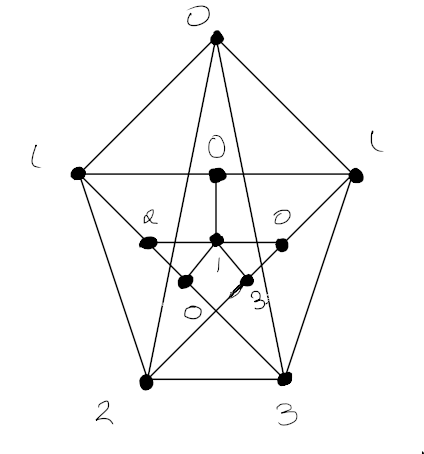
\includegraphics[scale=0.3]{Grafo10}
\end{center}

Ahora considere el siguiente subgrafo de $G$:

\begin{center}
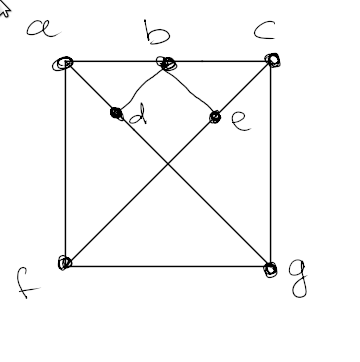
\includegraphics[scale=0.3]{Subgrafo10}
\end{center}

(Aquí los números denotan nombres de las aristas y no colores, como en el caso
anterior). Pues contiene a $C_3$ necesitamos al menos tres colores para
colorearlo propiamente. Asuma que existe un coloreo propio de tres colores. Los
dos $C_3$s se colorearán con los colores necesarios; por ejemplo, $c(a) = c(c) =
0, c(b) = 1, c(d) = c(e) = 2$. El único color disponible para $f$ es $1$; y si
se colorea a $f$ con $1$ no existe ningún color disponible para $g$ (y
viceversa). Es decir, no existe un coloreo propio de tres colores. 

El resultado anterior implica que $\chi(G) \geq 4$. Pero ya dimos un coloreo
propio de cuatro colores de $G$. Luego $\chi(G) = 4$.


\pagebreak 

\begin{problem}
    Igual que el anterior pero con un $C_7$.
\end{problem}

Es fácil notar que $\mathscr{G}$ da un coloreo propio de $4$ colores, con lo cual
$\chi(G) \leq 4$. Pues $C_7 \subseteq G$, $\chi(G) \geq 3$. Es decir, $\chi(G)
\in \left\{ 3, 4 \right\} $. Es fácil encontrar un subgrafo de $G$ que no puede
colorearse propiamente con $3$ colores, lo cual concluye la prueba.

\pagebreak 

\begin{problem}
    Sea $G = (V, E) $ un grafo tal que $\chi(H) < \chi(G)$ para todo $H
    \subseteq G$. Probar que $\chi(G) \leq \delta + 1$.
\end{problem}

Asuma que $\chi(G) > \delta + 1$. Esto implica que $\delta < \chi(G) - 1$. Sea
$G'$ el grafo inducido por un vértice de grado $\delta$ y todos sus vecinos. Es
trivial observar que en el peor caso este grafo tiene $\chi(G') = \delta + 1$,
Pues $G$ es crítico, tendríamos que $\delta + 1 < \chi(G)$, lo cual contradice
la hipótesis.

Pues existe al menos un caso que contradice la hipótesis, y la hipótesis es
general, la contradicción es general. Es decir, $\chi(G) \leq \delta + 1$.

\pagebreak
\subsection{Practico 2}

\begin{problem}
    Cambie la definición de network permitiendo que cada lado tenga dos
    capacidades asociades, $c_1(\overrightarrow{xy})$ y
    $c_2(\overrightarrow{xy})$, con $c_1(\overrightarrow{xy}) \leq
    c_2(\overrightarrow{xy})$ para todo $\overrightarrow{xy} \in E$. Cambie la
    definición de flujo agregando la restricción de que
    $c_{1}(\overrightarrow{xy}) \leq f(\overrightarrow{xy}) \leq
    c_2(\overrightarrow{xy})$.

    Encuentro una network donde pueda no existir ningún flujo de $s$ a $t$.
\end{problem}

Sea $\mathcal{N} = (V, E, c_1, c_2)$ una network bajo la nueva definición.
Queremos construir $\mathcal{N}$ de modo tal que no exista ninguna $f$ que
satisfaga simultáneamente las siguientes propiedades: 

\begin{quote}
    \begin{itemize}
        \item $c_1(\overrightarrow{xy}) \leq f(\overrightarrow{xy}) \leq c_2(\overrightarrow{xy})$
        \item $in_f(x) = out_f(x) ~ \forall x \in \left( V - \left\{ s, t \right\}  \right) $
        \item $out_f(s) \geq in_f(s) $
        \item $in_f(t) \geq out_f(t) $
    \end{itemize}
\end{quote}

\begin{problem}
    Sea $\mathcal{N} = (V, E, c)$ una network con max flow $\mathcal{M}$. Sea
    $\mathcal{N}' = (V, E, c')$ donde $c'(\overrightarrow{xy}) =
    c(\overrightarrow{xy}) + k$ para toda $\overrightarrow{xy} \in E$. Determine
    si el max flow $\mathcal{M}'$ de $\mathcal{N}'$ es mayor a $\mathcal{M}$ y
    (de serlo) cuánto.
\end{problem}

Sea $f$ un flujo maximal de $\mathcal{N}$; es decir, un flujo tal que $v(f) =
\mathcal{M}$. Luego $out_f(s) - in_f(s) = \mathcal{M}$ (por definición).

Sea $f'$ un flujo sobre $\mathcal{N}'$ definido como $f'(\overrightarrow{xy}) =
f(\overrightarrow{xy}) + k$ para todo $\overrightarrow{xy} \in E$, excepto
cuando $y = s$, donde se define simplemente como $f(\overrightarrow{xs})$. Observe que

\begin{align*}
    v(f') &= \sum_{x \in V \land \overrightarrow{sx} \in E}
    f'(\overrightarrow{sx}) - \sum_{x \in V \land  \overrightarrow{xs} \in E}
    f'(\overrightarrow{xs}) \\ 
    &= \sum_{\ldots} \left[ f(\overrightarrow{sx}) + k \right]  - \sum_{\ldots}
    \left[ f(\overrightarrow{xs})\right]  \\ 
    &= v(f) + kw  \\ 
    &= \mathcal{M} + kw \\ 
\end{align*}

donde $w$ es la cantidad de lados que salen de $s$. 
Esto basta para probar que el max flow de $\mathcal{N}'$ es al menos
$\mathcal{M} + k$, y aumenta proporcionalmente a la cantidad de lados que salen
de $s$.

\begin{problem}[Ejercicio 3]

    
\end{problem}

    Sea $\mathcal{N} = (V, E, c)$ una network tal que existen loops y lados
    bidireccionales y sea $\mathcal{N}' = (V, E', c)$ la misma network pero con todos los
    loops y lados bidireccionales removidos; es decir, $E' = E - \left\{
    \overrightarrow{xy} \in E : x = y \lor \overrightarrow{yx} \in E \right\} $.
    Sea $f'$ un flujo sobre $\mathcal{N}$. Observe que, si existen lados
    bidireccionales o loops que involucren a $s$, tenemos 

    \begin{align*}
        v(f) &= \sum_{\ldots} f(\overrightarrow{sx}) -
        \sum_{\ldots}f(\overrightarrow{xs}) \\ 
             &= \left[ \sum_{\ldots} f(\overrightarrow{sx}) +
                 \sum_{\text{bidirecciones}} f(\overrightarrow{sx}) +
                 f(\overrightarrow{ss}) \right] - \left[  \sum_{\ldots}
             f(\overrightarrow{xs}) + \sum_{\text{bidirecciones}} f(\overrightarrow{xs})+  f(\overrightarrow{ss}) \right] \\ 
             &= \sum_{\text{respecto a } E'} f(\overrightarrow{sx}) -
             \sum_{\text{respecto a } E'}f(\overrightarrow{xs}) \\ 
             &=v(f) \text{ respecto a  } \mathcal{N}'
    \end{align*}

En otras palabras, los loops y las bidirecciones no contribuyen al valor de un
flujo, y el valor de todo flujo $f$ en un grafo con loops y bidirecciones es
igual al valor de ese mismo flujo sobre el grafo sin loop y bidirecciones.
Observe que la identidad indica lo mismo en el sentido inverso; es decir $v(f)$
sobre $\mathcal{N}'$ equivale a $v(f)$ sobre $\mathcal{N}$.

Luego, si tenemos una caja negra que encuentra flujos maximales para grafos sin
loops y bidirecciones, simplemente la usamos para encontrar el flujo maximal de
$\mathcal{N}'$, y ese mismo flujo (cualquiera sea el valor que asigne a los
loops y bidirecciones) será maximal en $\mathcal{N}$.

\begin{problem}[Ejercicio 4]
    
\end{problem}

Usaremos $s$ para denotar la única fuente de la network que queremos construir,
y $s_1, \ldots, s_n$ las $n$ fuentes de la network dada. 

La primera cuestión obvia es que $\overrightarrow{sx}$ debe existir para todo
$x $ tal que $\overrightarrow{s_i x}$ existe. Es decir, si un nodo puede recibir
flujo de alguna de las $n$ fuentes del grafo original, la fuente de nuestro
grafo construido debe poder transferir flujo a ese nodo.

La segunda cuestión obvia es que si $\mathscr{I}$ es la cantidad total de flujo
que puede recibir $x$ desde las $n$ fuentes originales, la fuente $s$ de nuestro
grafo construido debe poder ser capaz de transferir $\mathscr{I}$ a $x$. Es
decir, $c(\overrightarrow{sx})$ debe hacerse igual a $c(\left\{ s_1, \ldots, s_n
\right\}, x )$. Es fácil ver que estas dos condiciones concluyen el problema. 

Transformar $k$ resumideros $t_1, \ldots, t_k$ en uno solo es análogo.

\begin{problem}[Ejercicio 6]
   Algoritmo: 

   
   \small
   \begin{quote}
   
   \begin{itemize}
       \item Buscar todos los cortes 
        \item Calcular sus capacidades 
        \item Retornar la menor capacidad
   \end{itemize}
   
   \end{quote}
   \normalsize
   

\end{problem}

Por max-flow min-cut, sabemos que este algoritmo devuelve el max flow. Deben
computarse todos los subconjuntos $S \subseteq V - \left\{ t \right\} $ que
contengan a $s$. Hay $2^{n}$ subconjuntos de $V$; si excluimos $t$, hay $2^{n -
1}$ subconjuntos de $V$; y si aseguramos que $s$ se encuentre en ellos, hay
$2^{n - 2}$.

Por cada uno de estos cortes, debemos computar su capacidad, lo cual involucra
sumar las capacidades de todos los lados desde el conjunto hacia afuera del
conjunto. Es evidente que $\frac{n(n-1)}{2}$, la máxima cantidad de lados, es
una cota a la cantidad de capacidades a sumar. Esto nos dice que la complejidad
del cálculo de las capacidades es \textit{a lo sumo} $O(n^2)$. Pues esto es
menor a la complejidad exponencial del primer paso, no hace falta considerarlo
más. 

El último paso (retornar la menor capacidad) también requiere $2^{n-1}$ pasos.
La complejidad del algoritmo es $O(2^{n-2})$.

\begin{problem}[Ejercicio 7]
    
\end{problem}

Por min-cut max-flow, el valor de cualquier flujo maximal es la capacidad del
corte minimal. En particular, $\mathcal{S} = \left\{ s \right\} \cup  \left\{ x
\in V : \exists f\text{-c.a.} \text{ de $s$ a $x$ }\right\} $ es un corte
minimal.

Si todos los lados tienen capacidad par, la suma de las
capacidades de los lados que van desde hacia fuera del corte minimal es una suma
par. $\blacksquare$



\end{document}



